% !TEX TS-program = lualatex
% !TEX encoding = UTF-8
\def\tenebrae{T}
\newcommand{\ifbook}[1]{#1}
\newcommand{\ifnotbook}[1]{}
%
\documentclass[12pt]{article} % use larger type; default would be 10pt
%\usepackage{hyperref}
% !TEX TS-program = lualatex
% !TEX encoding = UTF-8
% usual packages loading:
%\usepackage{luatextra}
%\usepackage{graphicx} % support the \includegraphics command and options
\usepackage{geometry} % See geometry.pdf to learn the layout options. There are lots.
\ifx\undefined\mywidth
    \geometry{letterpaper} % or letterpaper (US) or a5paper or....
\else
    \geometry{papersize={\mywidth,\myheight}}
\fi
\usepackage{expl3}
\let\luatexlocalrightbox\localrightbox
\let\luatexlocalleftbox\localleftbox
\usepackage{gregoriotex} % for gregorio score inclusion
\usepackage{import}

% If you use usual TeX fonts, here is a starting point:
%\usepackage{palatino}
%\input{glyphtounicode} \pdfglyphtounicode{f_f}{FB00} \pdfglyphtounicode{f_f_i}{FB03} \pdfglyphtounicode{f_f_l}{FB04}
%\pdfglyphtounicode{Q_u}{E048} \pdfglyphtounicode{O_e}{0152} \pdfglyphtounicode{o_e}{0153}
%\pdfgentounicode=1
% to change the font to something better, you can install the kpfonts package (if not already installed). To do so
% go open the "TeX Live Manager" in the Menu Start->All Programs->TeX Live 2010
% the additional width of the additional lines (compared to the width of the glyph they're associated with)
\grechangedim{additionallineswidth}{0.14584 cm}{scalable}%
% width of the additional lines, used only for the custos (maybe should depend on the width of the custos...)
% the width is the one for the custos at end of lines, the line for custos in the middle of a score is the same
% multiplied by 2.
\grechangedim{additionalcustoslineswidth}{0.09114 cm}{scalable}%
% null space
\grechangedim{zerowidthspace}{0 cm}{scalable}%
% space between glyphs in the same element
\grechangedim{interglyphspace}{0.06927 cm plus 0.00363 cm minus 0.00363 cm}{scalable}%
% space between an alteration (flat or natural) and the next glyph
\grechangedim{alterationspace}{0.07747 cm plus 0.01276 cm minus 0.00455 cm}{scalable}%
% space between a clef and a flat (for clefs with flat)
\grechangedim{clefflatspace}{0.05469 cm plus 0.00638 cm minus 0.00638 cm}{scalable}%
% space before a choral sign
\grechangedim{beforelowchoralsignspace}{0.04556 cm plus 0.00638 cm minus 0.00638 cm}{scalable}%
% when bolshifts are enabled, minimal space between a clef at the beginning of the line and a leading alteration glyph (should be larger than clefflatspace so that a flatted clef can be distinguished from a flat which is part of the first glyph on a line, but also smaller than spaceafterlineclef, the distance from the clef to the first notes)
\grechangedim{beforealterationspace}{0.1 cm}{scalable}%
% space between elements
\grechangedim{interelementspace}{0.06927 cm plus 0.00182 cm minus 0.00363 cm}{scalable}%
% larger space between elements
\grechangedim{largerspace}{0.10938 cm plus 0.01822 cm minus 0.00911 cm}{scalable}%
% space between elements in ancient notation
\grechangedim{nabcinterelementspace}{0.06927 cm plus 0.00182 cm minus 0.00363 cm}{scalable}%
% larger space between elements in ancient notation
\grechangedim{nabclargerspace}{0.10938 cm plus 0.01822 cm minus 0.00911 cm}{scalable}%
% space between elements which has the size of a note
\grechangedim{glyphspace}{0.21877 cm plus 0.01822 cm minus 0.01822 cm}{scalable}%
% space before custos
\grechangedim{spacebeforecustos}{0.1823 cm plus 0.31903 cm minus 0.0638 cm}{scalable}%
% space before punctum mora and augmentum duplex
\grechangedim{spacebeforesigns}{0.05469 cm plus 0.00455 cm minus 0.00455 cm}{scalable}%
% space after punctum mora and augmentum duplex
\grechangedim{spaceaftersigns}{0.08203 cm plus 0.0082 cm minus 0.0082 cm}{scalable}%
% space after a clef at the beginning of a line
\grechangedim{spaceafterlineclef}{0.27345 cm plus 0.14584 cm minus 0.01367 cm}{scalable}%
% minimal space between notes of different words
%\grechangedim{interwordspacenotes}{0.27 cm plus 0.15 cm minus 0.05 cm}{scalable}%
\grechangedim{interwordspacenotes}{0.27 cm plus 0.08 cm minus 0.05 cm}{scalable}%
% minimal space between notes of the same syllable.
% Warning: always keep minus to 0; also keep plus very low, or some words won't be hyphenated
%\grechangedim{intersyllablespacenotes}{0.24 cm plus 0.04cm minus 0cm}{scalable}%
\grechangedim{intersyllablespacenotes}{0.24 cm plus 0.04cm minus 0cm}{scalable}%
% minimal space between letters of different words. Makes sense to have
% the same plus and minus as interwordspacenotes.
%\grechangedim{interwordspacetext}{0.38 cm plus 0.15 cm minus 0.05 cm}{scalable}%
\grechangedim{interwordspacetext}{0.18 cm plus 0.08 cm minus 0.05 cm}{scalable}%
% Versions of interword spaces for euouae blocks
%\grechangedim{interwordspacenotes@euouae}{0.19 cm plus 0.1 cm minus 0.05 cm}{scalable}%
\grechangedim{interwordspacenotes@euouae}{0.13 cm plus 0.1 cm minus 0.05 cm}{1}%
%\grechangedim{interwordspacetext@euouae}{0.27 cm plus 0.1 cm minus 0.05 cm}{scalable}%
\grechangedim{interwordspacetext@euouae}{0.13 cm plus 0.1 cm minus 0.05 cm}{1}%
% space between notes of a bivirga or trivirga
\grechangedim{bitrivirspace}{0.06927 cm plus 0.00182 cm minus 0.00546 cm}{scalable}%
% space between notes of a bistropha or tristrophae
\grechangedim{bitristrospace}{0.06927 cm plus 0.00182 cm minus 0.00546 cm}{scalable}%
% space between two punctum inclinatum
\grechangedim{punctuminclinatumshift}{-0.03918 cm plus 0.0009 cm minus 0.0009 cm}{scalable}%
% space before puncta inclinata
\grechangedim{beforepunctainclinatashift}{0.05286 cm plus 0.00728 cm minus 0.00455 cm}{scalable}%
% space between a punctum inclinatum and a punctum inclinatum deminutus
\grechangedim{punctuminclinatumanddebilisshift}{-0.02278 cm plus 0.0009 cm minus 0.0009 cm}{scalable}%
% space between two punctum inclinatum deminutus
\grechangedim{punctuminclinatumdebilisshift}{-0.00728 cm plus 0.0009 cm minus 0.0009 cm}{scalable}%
% space between puncta inclinata, larger ambitus (range=3rd)
\grechangedim{punctuminclinatumbigshift}{0.07565 cm plus 0.0009 cm minus 0.0009 cm}{scalable}%
% space between puncta inclinata, larger ambitus (range=4th -or more?-)
\grechangedim{punctuminclinatummaxshift}{0.17865 cm plus 0.0009 cm minus 0.0009 cm}{scalable}%
% space for the bars (inside syllables)
%first for virgula and divisio minima
\grechangedim{spacearoundsmallbar}{0.1823 cm plus 0.22787 cm minus 0.00469 cm}{scalable}%
%then divisio minor
\grechangedim{spacearoundminor}{0.1823 cm plus 0.22787 cm minus 0.00469 cm}{scalable}%
%divisio major
\grechangedim{spacearoundmaior}{0.1823 cm plus 0.22787 cm minus 0.00469 cm}{scalable}%
%divisio finalis
\grechangedim{spacearoundfinalis}{0.1823 cm plus 0.22787 cm minus 0.00469 cm}{scalable}%
%a special space for finalis, for when it is the last glyph
\grechangedim{spacebeforefinalfinalis}{0.29169 cm plus 0.07292 cm minus 0.27345 cm}{scalable}%
% additional space that will appear around bars that are preceded by a custos and followed by a key.
\grechangedim{spacearoundclefbars}{0.03645 cm plus 0.00455 cm minus 0.0009 cm}{scalable}%
% space between the text and the text of the bar
\grechangedim{textbartextspace}{0.24611 cm plus 0.13672 cm minus 0.04921 cm}{scalable}%
% minimal space between a note and a bar
\grechangedim{notebarspace}{0.31903 cm plus 0.27345 cm minus 0.02824 cm}{scalable}%
% maximal space between two syllables for which we consider a dash is not needed
\grechangedim{maximumspacewithoutdash}{0.00 cm}{scalable}%
% an extensible space for the beginning of lines
\grechangedim{afterclefnospace}{0 cm plus 0.27345 cm minus 0 cm}{scalable}%
% space between the initial and the beginning of the score
\grechangedim{afterinitialshift}{0.2457 cm}{scalable}%
% space before the initial
\grechangedim{beforeinitialshift}{0.2457 cm}{scalable}%
% when bolshifts are enabled, minimum space between beginning of line and first syllable text
\grechangedim{minimalspaceatlinebeginning}{0.05 cm}{scalable}%
% space to force the initial width to.  Ignored when 0.
\grechangedim{manualinitialwidth}{0 cm}{scalable}%
% distance to move the initial up by
\grechangedim{initialraise}{0 cm}{scalable}%
% Space between lines in the annotation
\grechangedim{annotationseparation}{0.05cm}{scalable}%
% Amount to raise (positive) or lower (negative) the annotations from the default position (base line of top annotation aligned with top line of staff)
\grechangedim{annotationraise}{0cm}{scalable}%
% space at the beginning of the lines if there is no clef
\grechangedim{noclefspace}{0.1 cm}{scalable}%
% space around a clef change
\grechangedim{clefchangespace}{0.01768 cm plus 0.00175 cm minus 0.01768 cm}{scalable}%
%When \gre@clivisalignment is 2, this distance is the maximum length of the consonants after vowels for which the clivis will be aligned on its center.
\grechangedim{clivisalignmentmin}{0.3 cm}{scalable}%



%%%%%%%%%%%%%%%%%%
% vertical spaces
%%%%%%%%%%%%%%%%%%

% first, we have two spaces for the chironomic signs
\grechangedim{abovesignsspace}{0.8 cm}{scalable}%
\grechangedim{belowsignsspace}{0 cm}{scalable}%
% the amount to shift down:
% (a) low choral signs that are not lower than the note, regardless of whether
%     it's on a line or in a space
% (b) high choral signs and low choral signs that are lower than the note which
%     are in a space
\grechangedim{choralsigndownshift}{0.00911 cm}{scalable}%
% the amount to shift up:
% (a) high choral signs and low choral signs that are lower than the note which
%     are on a line
\grechangedim{choralsignupshift}{0.04556 cm}{scalable}%
% the space for the translation
\grechangedim{translationheight}{0.5 cm}{scalable}%
%the space above the lines
\grechangedim{spaceabovelines}{0.45576 cm plus 0.36461 cm minus 0.09114 cm}{scalable}%
%the space between the lines and the bottom of the text
\grechangedim{spacelinestext}{0.60617 cm}{scalable}%
%the space beneath the text
\grechangedim{spacebeneathtext}{0 cm}{scalable}%
% height of the text above the note line
\grechangedim{abovelinestextraise}{-0.1 cm}{scalable}%
% height that is added at the top of the lines if there is text above the lines (it must be bigger than the text for it to be taken into consideration)
\grechangedim{abovelinestextheight}{0.3 cm}{scalable}%
% an additional shift you can give to the brace above the bars if you don't like it
\grechangedim{braceshift}{0 cm}{scalable}%
% a shift you can give to the accentus above the curly brace
\grechangedim{curlybraceaccentusshift}{-0.05 cm}{scalable}%


%\def\greinitialformat#1{{\fontsize{37}{37}\selectfont #1}}
%small > footnotesize > scriptsize > tiny


% my stuff
\usepackage[garamond]{../mypackage}
% end my stuff

\setgrefactor{17}

%\marginsize{25pt}{25pt}{25pt}{30pt}
\usepackage{calc}
%\setlength\headsep{20pt}
%\setlength\footskip{15pt}
\setlength\headheight{15pt}
\setlength\headsep{22pt}
\ifx\undefined\tenebrae
    \geometry{outer=25pt,inner=25pt,top=22pt+\headsep+\headheight,bottom=25pt+\footskip}
\else
    \ifx\undefined\mywidth
        %had been .3 outer, .4 inner
        %let's try .75 for inner and .5 for outer
        %now let's go to .35 outer, .9 inner
        %this time let's try .4 and .85
        \ifbook{\geometry{outer=0.4in,inner=0.85in,top=25pt+\headsep+\headheight,bottom=25pt+\footskip,twoside=true}}
        \ifnotbook{\geometry{outer=0.625in,inner=0.625in,top=25pt+\headsep+\headheight,bottom=25pt+\footskip,twoside=true}}
    \else
        \setlength\headsep{0.25in}
        \setlength\footskip{0.3in}
        \geometry{outer=0.5in,inner=0.5in,top=0.25in+\headsep+\headheight,bottom=0.25in+\footskip,twoside=true}
    \fi
\fi

\pagestyle{fancy} % no header or footers
\let\oldheadrulewidth\headrulewidth
\renewcommand\headrulewidth{\ifnum\thepage=1
0pt
\else
\oldheadrulewidth
\fi}

\ifx\undefined\ifbook
    \newcommand{\ifbook}[1]{}
    \newcommand{\ifnotbook}[1]{#1}
\fi
\ifx\undefined\ifsmallbook
    \newcommand{\ifsmallbook}[1]{}
    \newcommand{\ifnotsmallbook}[1]{#1}
\fi
%\cfoot{\thepage}


\def\mypreface{
\thispagestyle{empty}
\begin{center}
\Huge Preface
\end{center}
\bigskip
All the chants found herein have been typeset based on those found in the Liber Usualis from 1961.

Most of the chant was already typeset by Andrew Hinkley and made easily available on http://gregobase.selapa.net.  So many thanks to them.  Also my brother Benjamin's gabc tools were also quite helpful and so I offer him my gratitude as well.  I also would like to thank Sean Connolly who composed the responsories for Good Friday.

April 2, 2014
Cincinnati, Ohio
}

\def\mycopyrightpage{
\vfill
First edition, 5 April 2014

All chant is based on those found in the Liber Usualis published in 1961.
\pagebreak
}

\def\mytitlepage{%
\thispagestyle{empty}
\def\dotting{\xleaders\hbox to 12pt{\hfil.\hfil}\hfill}
%\def\wdotting{\leaders\hbox to 3em{\hfil.\hfil}\hfill}
\def\wdotting{\hfill}
\vspace*{50pt}
\begin{center}{\addfontfeature{Numbers=Lining}%
\Huge \textsc{Tenebrae}
\vspace*{50pt}
\bigskip
\bigskip
\bigskip
}\end{center}
\pagebreak
}

\def\mytoc{%
\thispagestyle{empty}
%\vspace*{50pt}
\def\dotting{\xleaders\hbox to 12pt{\hfil.\hfil}\hfill}
%\def\wdotting{\leaders\hbox to 3em{\hfil.\hfil}\hfill}
\def\wdotting{\hfill}
\noindent
\huge\hfil Contents\hfil\\
\def\heading{Contents}

\vfil
\large
\noindent
\textsc{Maundy Thursday}\dotting \pageref{thursday-1}\\
\hspace*{4em}Resp. 1: In monte Olivéti\wdotting \pageref{in_monte_oliveti}, \pageref{in_monte_oliveti_poly}\\
\hspace*{4em}Resp. 2: Tristis est ánima mea\wdotting \pageref{tristis_est_anima_mea}, \pageref{tristis_est_anima_mea_poly}\\
\hspace*{4em}Resp. 3: Ecce vídimus eum\wdotting \pageref{resp3_ecce_vidimus}\\
\hspace*{2em}\textsc{2nd Nocturn}\dotting \pageref{thursday-2}\\
\hspace*{4em}Resp. 4: Amícus meus\wdotting \pageref{resp4_amicus_meus}\\
\hspace*{4em}Resp. 5: Judas mercátor\wdotting \pageref{resp5_judas_mercator}\\
\hspace*{4em}Resp. 6: Unus ex discípulis meis\wdotting \pageref{resp6_unus_ex_discipulis}\\
\hspace*{2em}\textsc{3rd Nocturn}\dotting \pageref{thursday-3}\\
\hspace*{4em}Resp. 7: Eram quasi agnus ínnocens\wdotting \pageref{resp7_eram_quasi_agnus}\\
\hspace*{4em}Resp. 8: Una hora\wdotting \pageref{resp8_una_hora}\\
\hspace*{4em}Resp. 9: Senióres pópuli\wdotting \pageref{resp9_seniores}\\
\hspace*{2em}\textsc{Lauds}\dotting \pageref{thursday-lauds}\\
\\
\vfil
\noindent
\textsc{Good Friday}\dotting \pageref{friday-1}\\
\hspace*{4em}Resp. 1: Omnes amíci mei\wdotting \pageref{omnes_amici_mei}, \pageref{omnes_amici_mei_poly}\\
\hspace*{4em}Resp. 2: Velum templi scissum est\wdotting \pageref{velum_templi_scissum_est}, \pageref{velum_templi_scissum_est_poly}\\
\hspace*{4em}Resp. 3: Vínea mea elécta\wdotting \pageref{resp3_vinea_mea}\\
\hspace*{2em}\textsc{2nd Nocturn}\dotting \pageref{friday-2}\\
\hspace*{4em}Resp. 4: Tamquam ad latrónem\wdotting \pageref{resp4_tamquam_ad_latronem}\\
\hspace*{4em}Resp. 5: Ténebræ factæ sunt\wdotting \pageref{resp5_tenebrae}\\
\hspace*{4em}Resp. 6: Animam meam diléctam\wdotting \pageref{resp6_animam_meam}\\
\hspace*{2em}\textsc{3rd Nocturn}\dotting \pageref{friday-3}\\
\hspace*{4em}Resp. 7: Tradidérunt me\wdotting \pageref{resp7_tradiderunt}\\
\hspace*{4em}Resp. 8: Jesum trádidit\wdotting \pageref{resp8_jesum_tradidit}\\
\hspace*{4em}Resp. 9: Caligavérunt óculi mei\wdotting \pageref{resp9_caligaverunt}\\
\hspace*{2em}\textsc{Lauds}\dotting \pageref{friday-lauds}\\
\\
\vfil
\pagebreak
\noindent
\textsc{Holy Saturday}\dotting \pageref{saturday-1}\\
\hspace*{4em}Resp. 1: Sicut ovis\wdotting \pageref{resp1_sicut_ovis}\\
\hspace*{4em}Resp. 2: Jerúsalem, surge\wdotting \pageref{resp2_jerusalem}\\
\hspace*{4em}Resp. 3: Plange quasi virgo\wdotting \pageref{resp3_plange}\\
\hspace*{2em}\textsc{2nd Nocturn}\dotting \pageref{saturday-2}\\
\hspace*{4em}Resp. 4: Recéssit pastor noster\wdotting \pageref{resp4_recessit_pastor}\\
\hspace*{4em}Resp. 5: O vos omnes\wdotting \pageref{o_vos_omnes}, \pageref{o_vos_omnes_poly}\\
\hspace*{4em}Resp. 6: Ecce quómodo móritur\wdotting \pageref{resp6_ecce_quomodo_moritur}\\
\hspace*{2em}\textsc{3rd Nocturn}\dotting \pageref{saturday-3}\\
\hspace*{4em}Resp. 7: Astitérunt reges terræ\wdotting \pageref{resp7_astiterunt_reges}\\
\hspace*{4em}Resp. 8: Æstimátus sum\wdotting \pageref{resp8_aestimatus_sum}\\
\hspace*{4em}Resp. 9: Sepúlto Dómino\wdotting \pageref{resp9_sepulto_domino}\\
\hspace*{2em}\textsc{Lauds}\dotting \pageref{saturday-lauds}\\
\\
\textsc{Tone for the Prophecy}\dotting \pageref{prophecytone}\\
\\
\textsc{Christus Factus Est}\dotting \pageref{christus_factus_est}\\
\vfil
\pagebreak
\normalsize
}


% here we begin the document
\begin{document}
%\mycopyrightpage
\mytitlepage
\mytoc
%\mytitlepage % filler page

%\let\olditem=\item
%\def\item#1{\parbox{\hsize}{\olditem #1}}

%
\includegraphics{in_monte_oliveti-1}%
\ifx\betweenLilyPondSystem \undefined
  \linebreak
\else
  \expandafter\betweenLilyPondSystem{1}%
\fi
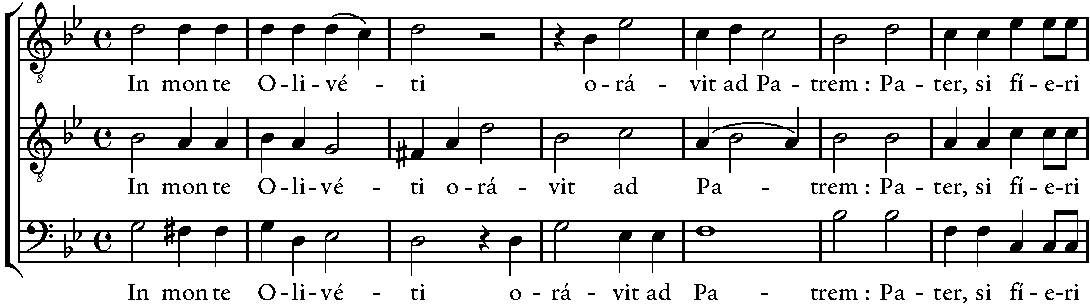
\includegraphics{in_monte_oliveti-2}%
\ifx\betweenLilyPondSystem \undefined
  \linebreak
\else
  \expandafter\betweenLilyPondSystem{2}%
\fi
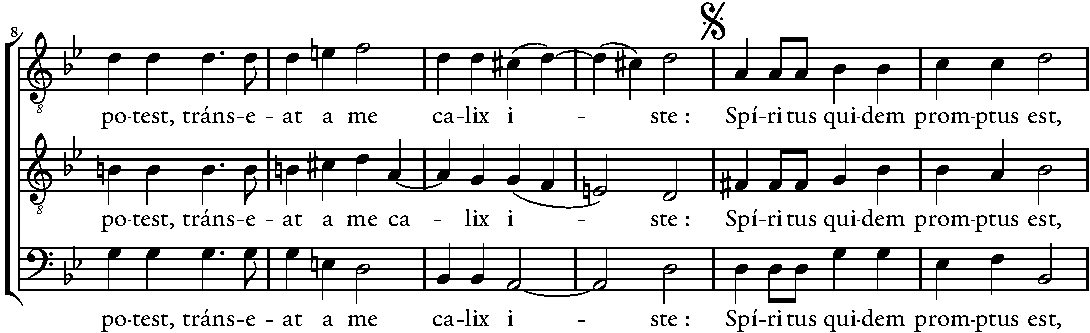
\includegraphics{in_monte_oliveti-3}%
\ifx\betweenLilyPondSystem \undefined
  \linebreak
\else
  \expandafter\betweenLilyPondSystem{3}%
\fi
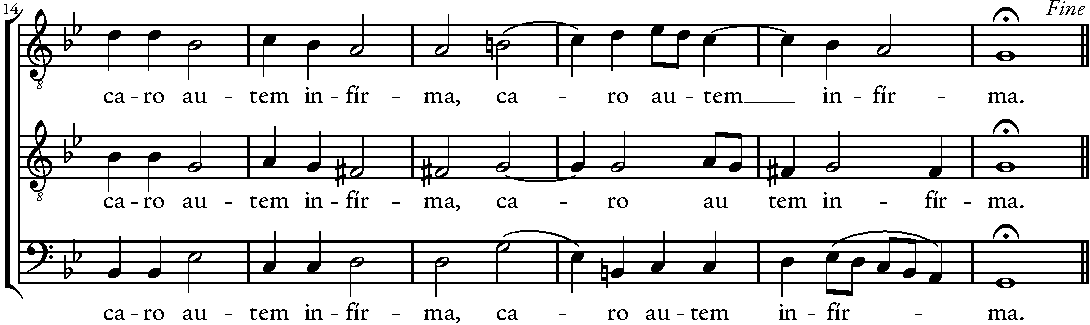
\includegraphics{in_monte_oliveti-4}%
\ifx\betweenLilyPondSystem \undefined
  \linebreak
\else
  \expandafter\betweenLilyPondSystem{4}%
\fi
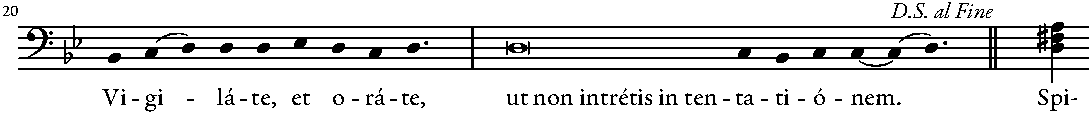
\includegraphics{in_monte_oliveti-5}%
% eof


%\ifnum 1=2{
% The title:
\vspace*{-50pt plus 20pt}
\begin{center}{\addfontfeature{Numbers=Lining}%
\huge \textsc{Maundy Thursday}

\bigskip
\normalsize\textsc{At Matins}
}\end{center}
%\vspace{-2ex}
%\bigskip

%\emph{The altar is prepared with cross and six lighted candles, but without ornament.}

\def\officehour{Matins}
\def\matinsnocturn{1st Nocturn}
\writeheading{In the 1st Nocturn}
%
\large
%\printgabc{1. Ant.}{8. c.}{Z}{an--zelus_domus_tuae--solesmes}
{
\def\preant{\setgrefactor{16}\normalsize}
\def\anttranslation{The zeal of Thy house hath consumed me, and the reproaches of them that reproach Thee, fell upon me.}
\def\psalmtranslationsmall{T}
\ifnotsmallbook{
    \def\lalinebreakafterthirtynine{T}
    \def\enlinebreakafterthirtyseven{T}
}
\def\prepsalm{\setgrefactor{14}\normalsize}
\ifsmallbook{
    \def\prepsalmverses{\bigskip}
}
\printpsalm{1}{68}{8c}{an--zelus_domus_tuae--solesmes}{Z}
}
%
\printseparation{}
\def\preant{\setgrefactor{17}\large}
\def\psalmtranslationsmall{T}
\def\anttranslation{Let them be turned back, and blush for shame: that think evil against me.}
\printpsalm{2}{69}{8c}{an--avertantur_retrorsum--solesmes}{A}
%
{
\def\preant{\setgrefactor{17}\large}
\def\psalmtranslationsmall{T}
\def\anttranslation{O my God, deliver me out of the hand of the sinner.}
\def\prepsalm{\setgrefactor{16}\normalsize\greblockcustos}
\def\lalinebreakaftertwentyone{T}
\def\prepsalmverses{\medskip}
\printpsalm{3}{70}{8c}{an--deus_meus_eripe_me--solesmes}{D}
\let\prepsalm=\undefined
}

\bigskip
\printvr{vr-avertanturRetrorsum}{Let them be turned back and put to shame.}{That intend evil against me.}

\bigskip\bigskip
Pater noster. \emph{in silence.}

\setgrefactor{14}
\medskip
\hspace{10ex}\textsc{lesson i}\hfill\emph{Chap. 1, 1-14}\hspace{10ex}

{\normalsize
\printgabc{}{}{I}{lesson1-thursday-IncipitLamentatioJeremiae}

\translation[\normalsize]{\emph{Aleph}. How doth the city sit solitary that was full of people! how is the mistress of the Gentiles become as a widow: the princess of provinces made tributary!
\emph{Beth}. Weeping she hath wept in the night, and her tears are on her cheeks: there is none to comfort her among all them that were dear to her: all her friends have despised her, and are become her enemies.
\emph{Ghimel}. Juda hath removed her dwelling place because of her affliction, and the greatness of her bondage: she hath dwelt among the nations, and she hath found no rest: all her persecutors have taken her in the midst of straits.
\emph{Daleth}. The ways of Sion mourn, because there are none that come to the solemn feast: all her gates are broken down: her priests sigh: her virgins are in affliction, and she is oppressed with bitterness.
\emph{He}. Her adversaries are become her lords, her enemies are enriched: because the Lord hath spoken against her for the multitude of her iniquities: her children are led into captivity: before the face of the oppressor.
Jerusalem, Jerusalem, return to the Lord thy God.}

\bigskip\bigskip\vfil

\printgabc{Resp. 1}{8.}{I}{re--in_monte_oliveti--solesmes}

\translation[\normalsize]{\Rbar{}. At the Mount of Olives He prayed unto the Father: Father, if it be possible, let this cup pass from Me!
* The spirit indeed is willing, but the flesh is weak.
\Vbar{}. Watch and pray, that ye enter not into temptation.
\Rbar{}. The spirit \dots{}}
}

\pagebreak
\begin{center}{\textsc{lesson ii}}\end{center}

{\normalsize
\printgabc{}{}{V}{lesson2-thursday-Vau}

\translation[\normalsize]{\emph{Vau}. And from the daughter of Sion all her beauty is departed: her princes are become like rams that find no pastures: and they are gone away without strength before the face of the pursuer.
\emph{Zain}. Jerusalem hath remembered the days of her affliction, and prevarication of all her desirable things which she had from the days of old, when her people fell in the enemy's hand, and there was no helper: the enemies have seen her, and have mocked at her sabbaths.
\emph{Heth}. Jerusalem hath grievously sinned, therefore is she become unstable: all that honoured her have despised her, because they have seen her shame: but she sighed and turned backward.
\emph{Teth}. Her filthiness is on her feet, and she hath not remembered her end: she is wonderfully cast down, not having a comforter: behold, O Lord, my affliction, because the enemy is lifted up.
Jerusalem, Jerusalem, return to the Lord thy God.}

\bigskip\bigskip

\needspace{4\baselineskip}
\printgabc{Resp. 2}{8.}{I}{re--tristis_est--solesmes}

\translation[\normalsize]{\Rbar{}. My soul is sorrowful even unto death: stay here and watch with me: now shall ye see the crowd that shall surround me: *
Ye shall take flight, and I will go to be offered up for you.
\Vbar{}. Behold, the hour draweth nigh, and the Son of man shall be delivered into the hands of sinners.
\Rbar{}. Ye shall flee \dots}
}

\bigskip
\begin{center}{\textsc{lesson iii}}\end{center}

{\normalsize
\printgabc{}{}{J}{lesson3-thursday-Jod}

\translation[\normalsize]{\emph{Jod}. The enemy hath put out his hand to all her desirable things: for she hath seen the Gentiles enter into her sanctuary, of whom thou gavest commandment that they should not enter into thy church.
\emph{Caph}. All her people sigh, they seek bread: they have given all their precious things for food to relieve the soul: see, O Lord, and consider, for I am become vile.
\emph{Lamed}. O all ye that pass by the way, attend, and see if there be any sorrow like to my sorrow: for he hath made a vintage of me, as the Lord spoke in the day of his fierce anger.
\emph{Mem}. From above he hath sent fire into my bones, and hath chastised me: he hath spread a net for my feet, he hath turned me back: he hath made me desolate, wasted with sorrow all the day long.
\emph{Nun}. The yoke of my iniquities hath watched: they are folded together in his hand, and put upon my neck: my strength is weakened: the Lord hath delivered me into their hand out of which I am not able to rise.
Jerusalem, Jerusalem, return to the Lord thy God.}

\bigskip\bigskip\vfil

\printgabc{Resp. 3}{5.}{E}{re--ecce_vidimus--solesmes}
\translation[\normalsize]{\Rbar{}. Behold, we have seen Him without comeliness or beauty: His look is gone from Him: He hath borne our sins and suffered for us:
* By His stripes are we healed.
\Vbar{}. Truly He hath borne our infirmities, and carried our sorrows:
\Rbar{}. By His stripes are we healed.
\Rbar{}. Behold, we have seen \dots}
}
%\pagebreak
\gdef\matinsnocturn{2nd Nocturn}
\label{thursday-2}
\writeheading[]{In the 2nd Nocturn}
%
\myantsize
\def\nogloriapatri{T}
%\def\preant{\myantsize}
%\def\preantafter{\myantsize} %15
\def\psalmtranslationsmall{F}
%\def\lalinebreakafterverse{14}
%\def\prepsalm{\mypsalmsize} %15
{%
\def\anttranslation{The Lord delivered the poor from the mighty: and the needy that had no helper.\pagebreak}
%\def\dontrepeatantiphon{T}
%\def\lalinebreakafterverse{12}
\printpsalm{1}{71}{7c}{an--liberavit_dominus--solesmes}{L}}
%
\printseparation
%\pagebreak
\bigskip\bigskip
{\def\anttranslation{The impious have thought and spoken wickedness: they have spoken iniquity on high.}%\vspace{-4pt}}
%\def\dontrepeatantiphon{T}
\def\lalinebreakafterverse{21}
\printpsalm{2}{72}{8c}{an--cogitaverunt_impii--solesmes}{C}}
%
%\printseparation
\pagebreak
%\bigskip\bigskip
%\def\prepsalmverses{\vspace{0pt minus 1pt}}
{\def\anttranslation{Arise, O Lord, and judge my cause.}%\vspace{-\baselineskip}}%
\def\lalinebreakafterverse{11}
\def\lalinebreakafterversex{11}
\printpsalm{3}{73}{1g}{an--exsurge_domine_et_judica--solesmes}{E}}
%psalm 70 - In te, Domine, speravi

%\bigskip
\pagebreak
\myvrsize
{\printvr{vr-DeusMeus}{O my God, deliver me from the hand of the sinner:}{And out of the hand of the law-breaker and of the unjust man.} %14
}
\bigskip
Pater noster. \emph{in silence.}

\mylessonsize
{\begin{center}
Ex Tractátu sancti Augustíni Epíscopi super Psalmos%
%\translation{From the treatise of St Augustine, Bishop, upon the psalms}
\end{center}
\hspace{10ex}\textsc{lesson iv}\hfill\emph{On Ps. 54, at verse 1}\hspace{10ex}
%\begin{parcolumns}[rulebetween,colwidths={1=0.45\linewidth}]{2}
\tenebraelesson{Exaudi,}{Deus, oratiónem meam, et ne despéxeris deprecatiónem meam~: inténde mihi, et exáudi me. Satagéntis, sollíciti, in tribulatióne pósiti, verba sunt ista. Orat multa pátiens, de malo liberári desíderans. Súperest ut videámus in quo malo sit~: et cum dícere cœperit, agnoscámus ibi nos esse~: ut communicáta tribulatióne, conjungámus oratiónem. Contristátus sum, inquit, in exercitatióne mea, et conturbátus sum. Ubi con\-\emph{tristátus}? ubi con\-\emph{turbátus}? In exercitatióne mea, inquit. Hómines malos, quos pátitur, commemorátus est~: eamdémque passiónem malórum hóminum, exercitatiónem suam dixit. Ne putétis gratis esse malos in hoc mundo, et nihil boni de illis ágere Deum. Omnis malus aut ídeo vivit, ut corrigátur; aut ídeo vivit, ut per illum bonus ex\textbf{er}ce\textbf{á}tur.}
{Hear my prayer, O God, and despise not my petition: attend to me and hear me. These are the words of a man travailing, anxious, and troubled. He prayeth in the midst of much suffering, longing to be rid of his affliction. Our part is to see what his affliction was, and when he hath told us, to acknowledge that we also suffer therefrom; so that, sharing in his trouble, we may also join in his prayer. I mourn in my exercise, he says, and am troubled. Wherein mourned he? Wherein was he troubled? He saith: In my exercise. He hath in mind the wicked that cause him affliction, and this suffering which came upon him at the hands of wicked men, he hath called his exercise. Think not that wicked men are in this world for nothing, and that God doth no good with them. Every wicked man liveth, either to repent, or to exercise the righteous.}
%\end{parcolumns}
\medskip
}
\vfil

\pagebreak
\myrespsize
{\label{resp4_amicus_meus}
\printgabc{Resp. 4}{8.}{A}{re--amicus_meus--solesmes}

\translationcolumns[\mytranslationsize]{\Rbar{}~My friend betrayed Me by the sign of a kiss: Whom I shall kiss, That is He, hold Him fast. This was the traitorous sign which he gave, who murdered with a kiss.
* Unhappy man, he relinquished the price of blood, and in the end hanged himself.
\Vbar{}~It had been good for that man, if he had not been born.
\Rbar{}~Unhappy man, he relinquished the price of blood~\dots}
}
\bigskip\bigskip
\pagebreak
\mylessonsize
{\begin{center}{\textsc{lesson v}}\end{center}
%\begin{parcolumns}[rulebetween,colwidths={1=0.44\linewidth}]{2}
\tenebraelesson{Utinam}{ergo qui nos modo exércent, convertántur, et nobíscum exerceántur~: tamen quámdiu ita sunt ut exérceant, non eos odérimus~: quia in eo quod malus est quis eórum, utrum usque in finem perseveratúrus sit, ignorámus. Et plerúmque cum tibi vidéris odísse inimícum, fratrem odísti, et nescis. Diábolus, et ángeli ejus in Scriptúris sanctis manifestáti sunt nobis, quod ad ignem ætérnum sint destináti. Ipsórum tantum desperánda est corréctio, contra quos habémus occúltam luctam~: ad quam luctam nos armat Apóstolus, dicens~: Non est nobis colluctátio advérsus carnem et sánguinem~: id est, non advérsus hómines, quos vidétis, sed advérsus príncipes, et potestátes, et rectóres mundi, tenebrárum harum. Ne forte cum dixísset, mundi, intellígeres dǽmones esse rectóres cæli et terræ, mundi dixit, tenebrárum harum~: mundi dixit amatórum mundi~: mundi dixit, impiórum et iniquórum~: mundi dixit, de quo dicit Evangélium~: Et mundus eum \textbf{non}~cog\textbf{nó}vit.}
{Would, therefore, that they who now exercise us were converted and exercised with us! Yet, while they are as they are, and exercise us, we will not hate them: for we know not of any one of them whether he will endure to the end in his sin. Yea, oftentimes, when thou deemest that thou hatest thine enemy, thou hatest thy brother, and knowest it not. The Holy Scriptures show us that the devil and his angels are already damned unto everlasting fire: their repentance alone is hopeless, against whom we wage a hidden strife. For which strife the Apostle would arm us, saying: We wrestle not against flesh and blood, (that is, not against men whom we see,) but against principalities, against powers, against the rulers of the darkness of this world. He saith not the rulers of this world, lest perchance thou shouldest deem that devils are the lords of heaven and earth; what he doth say is, rulers of the darkness of this world, of that world which they love who love the world, of that world wherein the ungodly and unrighteous do prosper, of that world, of which the Gospel saith: And the world knew Him not.}
%\end{parcolumns}
}

%\bigskip\bigskip
\pagebreak
\myrespsize
\greloadspaceconf{large-alt}
{\label{resp5_judas_mercator}
\printgabc{Resp. 5}{2.}{J}{re--judas_mercator--solesmes}

\translationcolumns[\mytranslationsize]{\Rbar{}~Judas, worst of traffickers, came to the Lord to kiss Him: He, as an innocent Lamb, refused not the kiss of Judas,
* Who, for a few pence, betrayed Christ to the Jews.
\Vbar{}~It had been better for him if he had not been born.
\Rbar{}~Who, for a few pence, betrayed Christ to the Jews.}
}

%\needspace{10\baselineskip}
\bigskip%\bigskip

\greloadspaceconf{large}
\mylessonsize
{\begin{center}{\textsc{lesson vi}}\end{center}
%\begin{parcolumns}[rulebetween,colwidths={1=0.432\linewidth}]{2}
\tenebraelesson[\columnratio{0.55}]{Quóniam}{vidi iniquitátem et contradictiónem in civitáte. Atténde glóriam crucis ipsíus. Jam in fronte regum crux illa fixa est, cui inimíci insultavérunt. Efféctus probávit virtútem~: dómuit orbem non ferro, sed ligno. Lignum crucis contuméliis dignum visum est inimícis, et ante ipsum lignum stantes caput agitábant, et dicébant~: Si Fílius Dei est, descéndat de cruce. Extendébat ille manus suas ad pópulum non credéntem, et contradicéntem. Si enim justus est, qui ex fide vivit; iníquus est, qui non habet fidem. Quod ergo hic ait, iniquitátem~: perfídiam intéllige. Vidébat ergo Dóminus in civitáte iniquitátem et contradictiónem, et extendébat manus suas ad pópulum non credéntem, et contradicéntem~: et tamen et ipsos exspéctans dicébat~: Pater, ignósce illis, quia nésci\textbf{unt} quid \textbf{fá}ciunt.}
{I have seen iniquity and strife in the city. Behold, the glory of the Cross. That Cross is established now above the brows of kings, which once enemies did deride. The end hath shown the measure of its power: He hath conquered the world, not with a sword, but with wood. The enemies of God thought the Cross a meet object of insult and ridicule, yea, they stood before it, wagging their heads and saying: If He be the Son of God, let Him come down from the Cross! And He stretched forth His Hands unto a disobedient and gainsaying people. If he is just which liveth by faith, he is unjust that hath not faith. Therefore where is written iniquity we may understand unbelief. The Lord therefore saith that He saw iniquity and strife in the city, and that He stretched forth His Hands unto that disobedient and gainsaying people, and yet, looking upon the very same, He said: Father, forgive them, for they know not what they do.}
%\end{parcolumns}
}
\bigskip\bigskip
\myrespsize
{\label{resp6_unus_ex_discipulis}
\printgabc{Resp. 6}{8.}{U}{re--unus_ex_discipulis--solesmes}
}
{
\translationcolumns[\mytranslationsize]{\Rbar{}~One of My disciples will betray Me today. Woe unto him by whom I am betrayed!
* It had been better for him if he had not been born.
\Vbar{}~He that dippeth his hand with Me in the dish, the same will deliver Me into the hands of sinners.
\Rbar{}~It had been better~\dots{}
\Rbar{}~One of My~\dots}
}
\pagebreak
\myantsize
%\bigskip
\def\matinsnocturn{3rd Nocturn}
\label{thursday-3}
\writeheading{In the 3rd Nocturn}
%
\large
{
%\printgabc{1. Ant.}{8. c.}{Z}{an--zelus_domus_tuae--solesmes}
\def\nogloriapatri{T}
\def\preant{\setgrefactor{17}\large}
\let\preantafter=\undefined
\def\anttranslation{I said unto the wicked: Speak not wickedness against God.}
\def\prepsalmverses{\vspace{-0.5\baselineskip}}
\def\psalmtranslationsmall{T}
\def\prepsalm{\setgrefactor{15}\normalsize}
\printpsalm{1}{74}{7c}{an--dixi_iniquis--solesmes}{D}
}
%
%\printseparation
\pagebreak
{
\def\preant{\setgrefactor{17}\large}
\let\preantafter=\undefined
\def\psalmtranslationsmall{T}
\def\prepsalm{\normalsize}
\def\anttranslation{The earth trembled and was still, when God arose in judgment.}
\printpsalm{2}{75}{8c}{an--terra_tremuit--solesmes}{T}
}
%
%\printseparation
\pagebreak
{
\def\preant{\setgrefactor{17}\large}
\def\prepsalm{\setgrefactor{14}\normalsize}
\let\preantafter=\undefined
\def\lalinebreakafterverse{17}
\def\prepsalmverses{\vspace{-0.5\baselineskip}}
\def\psalmtranslationsmall{T}
%\def\dontrepeatantiphon{T}
\def\anttranslation{In the day of my tribulation I sought God with my hands.}
\printpsalm{3}{76}{7a}{an--in_die_tribulationis--solesmes}{I}
}

\bigskip%\pagebreak
\bigskip
{
	%\def\vrnospace{T}
	\printvr{vr-ExsurgeDomine}{Arise, O Lord.}{And judge my cause.}
}

\bigskip
Pater noster. \emph{in silence.}

\begin{center}
De Epístola prima beáti Pauli Apóstoli ad Corínthios
%\translation{From the first epistle of St Paul the Apostle to the Corinthians}
\end{center}
{
\hspace{10ex}\textsc{lesson vii}\hfill\emph{Chap. 11, 17-34}\hspace{10ex}
\begin{parcolumns}[rulebetween,colwidths={1=0.5\linewidth}]{2}
\lesson{Hoc autem præcípio~: non laudans quod non in mélius, sed in detérius convenítis.
Primum quidem conveniéntibus vobis in Ecclésiam, áudio scissúras esse inter vos, et ex parte credo.
Nam opórtet et hǽreses esse, ut et qui probáti sunt, manifésti fiant in vobis.
Conveniéntibus ergo vobis in unum, jam non est Domínicam cenam manducáre.
Unusquísque enim suam cenam præsúmit ad manducándum, Et álius quidem ésurit, álius autem ébrius est.
Numquid domos non habétis ad}{manducándum, et \emph{bibéndum}? aut Ecclésiam Dei contémnitis, et confúnditis eos, qui \emph{non habent}? Quid di\-\emph{cam vobis}? \emph{Laudo vos}? In \textbf{hoc} non \textbf{lau}do.}
{Now this I ordain: not praising you, that you come together not for the better, but for the worse.
For first of all I hear that when you come together in the church, there are schisms among you; and in part I believe it.
For there must be also heresies: that they also, who are approved, may be made manifest among you.
When you come therefore together into one place, it is not now to eat the Lord's supper.
For every one taketh before his own supper to eat. And one indeed is hungry and another is drunk.
What, have you not houses to eat and to drink in? Or despise ye the church of God; and put them to shame that have not? What shall I say to you? Do I praise you? In this I praise you not.}
\end{parcolumns}
\setgrefactor{14}
\medskip

\bigskip\bigskip

\setgrefactor{17}
\needspace{12\baselineskip}
\printgabc{Resp. 7}{7.}{E}{re--eram_quasi_agnus--solesmes}

\translationcolumns[\normalsize]{\Rbar{}~I was like an innocent lamb: I was led to the sacrifice and I knew it not; mine enemies conspired against me, saying
* Come, let us put (poison of a deadly) tree into his bread, and root him out of the land of the living.
\Vbar{}~All mine enemies devised my hurt against me: they uttered a wicked speech against me, saying:
\Rbar{}~Come, let us put (poison of a deadly) tree into his bread, and root him out of the land of the living.}
}

%\bigskip%\bigskip
\vspace{-9pt}
\begin{center}{\textsc{lesson viii}}\end{center}
\vspace{-6pt}

\begin{parcolumns}[rulebetween,colwidths={1=0.5\linewidth}]{2}
\lesson{Ego enim accépi a Dómino quod et trádidi vobis, quóniam Dóminus Jesus, in qua nocte tradebátur, accépit panem,
et grátias agens fregit, et dixit~: «Accípite et manducáte~: hoc est corpus meum, quod pro vobis tradétur~: hoc fácite in meam commemoratiónem».
Simíliter et cálicem, postquam cenávit, dicens~: «Hic calix novum testaméntum est in meo sánguine~: hoc fácite, quotiescúmque bibétis, in meam commemoratiónem».
Quotiescúmque enim manducábitis panem hunc, et cálicem bibétis~: mortem Dómini}{annuntiábitis, \textbf{do}nec \textbf{vé}niat.}
{For I have received of the Lord that which also I delivered unto you, that the Lord Jesus, the same night in which he was betrayed, took bread.
And giving thanks, broke, and said: Take ye, and eat: this is my body, which shall be delivered for you: this do for the commemoration of me.
In like manner also the chalice, after he had supped, saying: This chalice is the new testament in my blood: this do ye, as often as you shall drink, for the commemoration of me.
For as often as you shall eat this bread, and drink the chalice, you shall show the death of the Lord, until he come.}
\end{parcolumns}

\bigskip\bigskip
{
\needspace{12\baselineskip}
\printgabc{Resp. 8}{7.}{U}{re--una_hora--solesmes}

\translationcolumns[\normalsize]{\Rbar{}~Could ye not watch with Me one hour, ye that called one on the other to die for Me?
* Or see ye not Judas, how he sleepeth not, but maketh haste to betray Me to the Jews?
\Vbar{}~Why sleep ye? Rise, and pray, lest ye enter into temptation.
\Rbar{}~Or see ye not Judas, how he sleepeth not, but maketh haste to betray Me to the Jews?}%
}%
\vspace{-6pt}
%\pagebreak
%\bigskip%\bigskip
\begin{center}{\textsc{lesson ix}}\end{center}
\vspace{-10pt}
\begin{parcolumns}[rulebetween,colwidths={1=0.49\linewidth}]{2}
\lesson{Itaque quicúmque manducáverit panem hunc vel bíberit cálicem Dómini indígne, reus erit córporis et sánguinis Dómini.
Probet autem seípsum homo~: et sic de pane illo edat et de cálice bibat.
Qui enim mandúcat et bibit indígne, judícium sibi mandúcat et bibit; non dijúdicans corpus Dómini.
Ideo inter vos multi infírmi et imbecílles, et dórmiunt multi.
Quod si nosmetípsos dijudicarémus, non útique judicarémur.
Dum judicámur autem, a Dómino corrípimur, ut non cum hoc mundo damnémur.
Itaque, fratres mei, cum convenítis ad manducándum, ínvicem exspectáte.
Si quis ésurit, domi mandúcet~: ut non in judícium conveniátis. Cétera autem,}{cum véne\textbf{ro}, dis\textbf{pó}nam.}
{Therefore whosoever shall eat this bread, or drink the chalice of the Lord unworthily, shall be guilty of the body and blood of the Lord.
But let a man prove himself: and so let him eat of that bread, and drink of the chalice.
For he that eateth and drinketh unworthily, eateth and drinketh judgment to himself, not discerning the body of the Lord.
Therefore are there many infirm and weak among you, and many sleep.
But if we would judge ourselves, we should not be judged.
But whilst we are judged, we are chastised by the Lord, that we be not condemned with this world.
Wherefore, my brethren, when you come together to eat, wait for one another.
If any man be hungry, let him eat at home; that you come not together unto judgment. And the rest I will set in order, when I come.}
\end{parcolumns}\vspace*{-20pt}
\pagebreak
\bigskip\bigskip
{
\needspace{4\baselineskip}
\printgabc{Resp. 9}{1.}{S}{re--seniores--solesmes}

\translationcolumns[\normalsize]{\Rbar{}~The elders of the people consulted
* That they might take Jesus by subtlety, and kill Him: they came out, as against a thief, with swords and clubs.
\Vbar{}~The chief Priests and the Pharisees gathered a council.
\Rbar{}~That they might take Jesus by subtlety, and kill Him: they came out, as against a thief, with swords and clubs.
\Rbar{}~The elders of the people~\dots}
}
%\pagebreak
%\medskip
\needspace{4\baselineskip}
%\bigskip\bigskip
\label{thursday-lauds}
\writeheading{At Lauds}
\let\matinsnocturn=\undefined
\def\officehour{Lauds}
%
\large
\def\nogloriapatri{T}
{
\def\preant{\grechangestaffsize{17}\large}
\let\preantafter=\undefined
\def\anttranslation{Be Thou justified in Thy words, O Lord, and do Thou overcome when judged.}
\def\psalmtranslationsmall{T}
\def\lalinebreakafterverse{5}
\printpsalm{1}{50}{8G}{an--justificeris_domine--solesmes}{J}
}
%
\printseparation
%\pagebreak
{
\def\preant{\grechangestaffsize{17}\large}
\def\preantafter{\grechangestaffsize{15}\normalsize}
\def\prepsalm{\grechangestaffsize{15}\normalsize}
\def\psalmtranslationsmall{T}
\def\dontrepeatantiphon{T}
\def\anttranslation{The Lord was led as a sheep to the slaughter, and opened not His mouth.}
\printpsalm{2}{89}{2D}{an--dominus_tamquam_ovis--solesmes}{D}
\let\prepsalm=\undefined
}
%
\printseparation
%\pagebreak
{
\def\preant{\grechangestaffsize{17}\large}
\let\preantafter=\undefined
\def\psalmtranslationsmall{T}
\def\anttranslation{My heart is broken within me: all my bones have trembled.}
\printpsalm{3}{35}{8G}{an--contritum_est_cor_meum--solesmes}{C}
}
%
\needspace{8\baselineskip}
\printseparation
{
\def\preant{\grechangestaffsize{17}\large}
\let\preantafter=\undefined
\def\psalmtranslationsmall{T}
\def\canticleof{Moses}
\def\canticleverses{Exod. 15, 1-19}
\def\prepsalm{\normalsize\grechangestaffsize{15}\greseteolcustos{manual}}
%\def\lalinebreakafterfifteen{T}
%\def\lalinebreakafterverse{14}
%\def\lalinebreakafterversex{14}
\printpsalm{4}{exod15}{4A}{an--exhortatus_es--solesmes}{E}
}
\let\canticleof=\undefined
\let\canticleverses=\undefined
\let\prepsalm=\undefined
%
\printseparation
%\pagebreak
{
\def\preant{\grechangestaffsize{17}\large}
\let\preantafter=\undefined
\def\psalmtranslationsmall{T}
\def\anttranslation{He was offered up because He willed it and He bore our sins.}
\def\prepsalm{\normalsize}
%\def\lalinebreakafterverse{3}
%\def\lalinebreakafterversex{3}
\printpsalm{5}{146}{2D}{an--oblatus_est--solesmes}{O}
\let\prepsalm=\undefined
}
\bigskip\bigskip
{
%\def\vrnospace{T}
\greseteolcustos{manual}
\printvr[\grechangestaffsize{15}\normalsize]{vr-HomoPacisMeae}{The man of my peace, in whom I trusted:}
{Who ate my bread, hath treacherously plotted against me.}
}

%\bigskip
\pagebreak
%\printgabc{At Bened.}{Ant. 1. g}{T}{an--traditor_autem--solesmes}
\def\magsolemn{T}
\def\prerepeatantiphon{\medskip}
\def\preverses{
  \grechangestaffsize{15}\normalsize
}
\def\preant{\large\grechangestaffsize{17}}
\def\anttranslation{\normalsize The traitor gave them a sign, saying: He whom I shall kiss, That Same is He: hold Him fast.}
\normalsize
\printmag[Benedictus]{1g}{T}{an--traditor_autem--solesmes}
%{1g}{an--traditor_autem--solesmes}{T}

%\emph{The candles on the triangular candlestick having been extinguished as has already been explained, the one at the top of the triangle alone remains lighted.  During the Canticle \emph{Benedíctus.} the candles on the altar are likewise extinguished one by one, from each side alternately, at every second verse, so that by the last verse all are extinguished.  All other lights and lamps in the church are also put out.}
\emph{After the repetition of the Antiphon at the \emph{Benedíctus}, all kneel and sing :}
\medskip
{\large\grechangestaffsize{17}
\printgabc{Ant.}{5.}{C}{../Tenebrae/an--christus_factus_est--solesmes_thursday}
}

\bigskip\bigskip

\emph{When the antiphon \emph{Christus fáctus est} is finished, \emph{Páter nóster} is said, in silence throughout.}

\emph{Then is sung, without \emph{Orémus}, to the ferial tone \emph{B} (or the ancient simple tone) :}

\bigskip
\bigskip

\begin{parcolumns}[rulebetween]{2}
\colchunk{\dropcap{latin}{Respice, quǽsumus, } Dómine, super hanc famíliam tuam,~† pro qua Dóminus noster Jesus Christus non dubitávit mánibus tradi nocéntium,~* et crucis subíre torméntum.
\emph{And in silence~:}
Qui tecum vivit et regnat in unitáte\dots{}}
\selectlanguage{american}
\colchunk{\dropcap{american}{Look down, we beseech thee, } O Lord, on this thy family, for which our Lord Jesus Christ did not hesitate to be delivered up into the hands of wicked men, and to suffer the torment of the Cross.}\end{parcolumns}
%}\fi
%\ifnum 1=2{
% The title:
\vspace*{-50pt plus 20pt}
\begin{center}{\addfontfeature{Numbers=Lining}%
\huge \textsc{Good Friday}

\bigskip
\normalsize\textsc{At Matins}
}\end{center}
%\vspace{-2ex}
%\bigskip

%\emph{The altar should be completely bare, and without crucifix or candles.}

\def\officehour{Matins}
\def\matinsnocturn{1st Nocturn}
\writeheading{In the 1st Nocturn}
%
\large
%\printgabc{1. Ant.}{8. c.}{Z}{an--zelus_domus_tuae--solesmes}
{
\def\preant{\setgrefactor{17}\large}
\def\prepsalm{\normalsize}
\def\anttranslation{The kings of the earth stood up, and the princes met together, against the Lord, and against His Anointed.}
\def\psalmtranslationsmall{T}
\def\prerepeatantiphon{\vspace{-20pt}}
\printpsalm{1}{2}{8G}{an--astiterunt_reges--solesmes}{A}
}
%
{
\def\preant{\setgrefactor{17}\large}
\def\prepsalm{\normalsize\setgrefactor{15}}
\def\psalmtranslationsmall{T}
\def\anttranslation{They parted my garments amongst them, and upon my vesture they cast lots.}
\printpsalm{2}{21}{8G}{an--diviserunt_sibi--solesmes}{D}
\let\prepsalm=\undefined
}
\bigskip
%
{
\def\preant{\setgrefactor{17}\large}
%\def\preantafter{\setgrefactor{15}\normalsize}
%\def\dontrepeatantiphon{T}
\def\psalmtranslationsmall{T}
\def\anttranslation{False witnesses are risen up against me, and iniquity hath belied itself.}
\def\prepsalm{\setgrefactor{16}\normalsize}
\printpsalm{3}{26}{8G}{an--insurrexerunt_in_me--solesmes}{I}
\let\prepsalm=\undefined
}

\bigskip
{
%\def\vrnospace{T}
\printvr[\normalsize]{vr-diviserunt}
{They parted my garments among them.}
{And upon my vesture they cast lots.}
}

\bigskip
Pater noster. \emph{in silence.}

\bigskip\bigskip
\hspace{10ex}\textsc{lesson i}\hfill\emph{Chap. 2, 8-15}\hspace{10ex}

{\normalsize\setgrefactor{14}
\printgabc{}{}{D}{lesson1-friday-DeLamentationeJeremiae}

\translationcolumns[\normalsize]{\emph{Heth}. The Lord hath purposed to destroy the wall of the daughter of Sion: He hath stretched out His line, and hath not withdrawn His hand from destroying: and the bulwark hath mourned, and the wall hath been destroyed together.
\emph{Teth}. Her gates are sunk into the ground: He hath destroyed, and broken her bars: her king and her princes are among the Gentiles: the law is no more, and her prophets have found no vision from the Lord.
\emph{Jod}. The ancients of the daughter of Sion sit upon the ground, they have held their peace: they have sprinkled their heads with dust, they are girded with haircloth, the virgins of Jerusalem hang down their heads to the ground.
\emph{Caph}. Mine eyes have failed with weeping, my bowels are troubled: my liver is poured out upon the earth, for the destruction of the daughter of my people, when the children, and the sucklings fainted away in the streets of the city.
Jerusalem, Jerusalem, return to the Lord thy God.}
}

\printseparation
%\bigskip

{
\setgrefactor{17}
\printgabc{Resp. 1}{3.}{O}{re--omnes_amici_mei--solesmes}

\translationcolumns[\normalsize]{\Rbar{}. All my friends have forsaken me, and they that lay wait for me have prevailed against me; he whom I loved hath betrayed me.
* And men of terrible countenance, piercing me with a cruel wound, have given me vinegar to drink.
\Vbar{}. They cast me out among the wicked, and spared not my soul.
\Rbar{}. And men of terrible countenance \dots{}}
}

\pagebreak
\begin{center}{\textsc{lesson ii}}\end{center}

{\normalsize\setgrefactor{14}
\printgabc{}{}{L}{lesson2-friday-Lamed}

\translationcolumns[\normalsize]{\emph{Lamed}. They said to their mothers: Where is corn and wine? when they fainted away as the wounded in the streets of the city: when they breathed out their souls in the bosoms of their mothers.
\emph{Mem}. To what shall I compare thee? or to what shall I liken thee, O daughter of Jerusalem? to what shall I equal thee, that I may comfort thee, O virgin daughter of Sion? for great as the sea is thy destruction: who shall heal thee?
\emph{Nun}. thy prophets have seen false and foolish things for thee: and they have not laid open thine iniquity, to excite thee to penance: but they have seen for thee false revelations and banishments.
\emph{Samech}. All they that passed by the way have clapped their hands at thee: they have hissed and wagged their heads at the daughter of Jerusalem, saying: Is this the city of perfect beauty, the joy of all the earth?
Jerusalem, Jerusalem, return to the Lord thy God.}
}

\bigskip\bigskip
\pagebreak

{\setgrefactor{17}
\printgabc{Resp. 2}{2.}{V}{re--velum_templi--solesmes}

\translationcolumns[\normalsize]{\Rbar{}. The veil of the Temple was rent,
* And all the earth did quake: the thief on the cross cried, saying: Lord, remember me when Thou comest into Thy kingdom!
\Vbar{}. The rocks were rent and the graves opened, and many bodies of the saints, which slept, arose.
\Rbar{}. And all the earth \dots}
}

\bigskip
\pagebreak
\hspace{10ex}\textsc{lesson iii}\hfill\emph{Chap. 3, 1-9}\hspace{10ex}

{\normalsize\setgrefactor{14}
\printgabc{}{}{A}{lesson3-friday-Aleph}

\translationcolumns[\normalsize]{\emph{Aleph}. I am the man that see my poverty by the rod of his indignation.
\emph{Aleph}. He hath led me, and brought me into darkness, and not into light.
\emph{Aleph}. Only against me he hath turned, and turned again his hand all the day.
\emph{Beth}. My skin and my flesh he hath made old, he hath broken my bones.
\emph{Beth}. He hath built round about me, and he hath compassed me with gall and labour.
\emph{Beth}. He hath set me in dark places as those that are dead for ever.
\emph{Ghimel}. He hath built against me round about, that I may not get out: he hath made my fetters heavy.
\emph{Ghimel}. Yea, and when I have cried and entreated, he hath shut out my prayer.
\emph{Ghimel}. He hath shut up my ways with square stones, he hath turned my paths upside down
Jerusalem, Jerusalem, return to the Lord thy God.}
}
%
%\bigskip\bigskip
%\bigskip%\bigskip
\bigskip
%
{\setgrefactor{17}
\printgabc{Resp. 3}{8.}{V}{re--vinea_mea--solesmes}
\translationcolumns[\normalsize]{\Rbar{}. O my chosen vine, I planted thee:
* How then art thou turned to bitterness, that thou shouldst crucify me, and release Barabbas?
\Vbar{}. I fenced thee, and gathered out the stones from thee, and built a tower.
\Rbar{}. How then art thou \dots{}
\Rbar{}. O my chosen vine \dots}
}
%\pagebreak
%\needspace{4\baselineskip}
\writeheading{In the 2nd Nocturn}
\def\matinsnocturn{2nd Nocturn}
%
\large
%\printgabc{1. Ant.}{8. c.}{Z}{an--zelus_domus_tuae--solesmes}
\def\nogloriapatri{T}
{
\def\preant{\setgrefactor{17}\large}
\def\prepsalm{\setgrefactor{14}\normalsize}
\def\prepsalmverses{\vspace{-10pt}}
%\def\dontrepeatantiphon{T}
\def\psalmtranslationsmall{T}
%\def\lalinebreakafterverse{16}
%\def\enlinebreakaftersixteen{T}
\def\anttranslation{They used violence that sought my soul.}
\printpsalm{1}{37}{8G}{an--vim_faciebant--solesmes}{V}
}
%
\printseparation
\bigskip
{
\def\preant{\setgrefactor{17}\large}
\def\preantafter{\setgrefactor{17}\normalsize}
\def\psalmtranslationsmall{T}
\def\prepsalm{\normalsize}
%\def\enlinebreakafternine{T}
\def\anttranslation{Let them be confounded and put to shame, that seek after my soul, to take it.}
\printpsalm{2}{39}{4A}{an--confundantur_et_revereantur--solesmes}{C}
}
%
\printseparation
%\pagebreak
{
\def\preant{\setgrefactor{17}\large}
\def\prepsalm{\normalsize\setgrefactor{15}}
\def\prepsalmverses{\vspace{-14pt}}
%\def\dontrepeatantiphon{T}
\def\psalmtranslationsmall{T}
\def\anttranslation{Strangers have risen up against me, and the mighty have sought after my soul.}
\printpsalm{3}{53}{4A}{an--alieni_insurrexerunt--solesmes}{A}
\let\prepsalm=\undefined
}
%psalm 70 - In te, Domine, speravi

\medskip
{\def\vrnospace{T}
\printvr[\setgrefactor{15}\normalsize]{vr-insurrexerunt}
{False witnesses are risen up against me.}
{And iniquity hath belied itself.}
}

\bigskip
Pater noster. \emph{in silence.}

\pagebreak
\begin{center}
Ex Tractátu sancti Augustíni Epíscopi super Psalmos
%\translation{From the treatise of St Augustine, Bishop, upon the psalms}
\end{center}
\hspace{10ex}\textsc{lesson iv}\hfill\emph{On Ps. 63, at verse 2}\hspace{10ex}

\ifnotsmallbook{
\ifx\undefined\useparacol
\begin{parcolumns}[rulebetween,colwidths={1=240pt}]{2}
\else
\begin{columns}
\fi
}
\ifsmallbook{\begin{columns}}
\lesson[\normalsize]{Protexísti me, Deus, a convéntu malignántium, a multitúdine operántium iniquitátem. Jam ipsum caput nostrum intueámur. Multi mártyres tália passi sunt, sed nihil sic elúcet, quómodo caput mártyrum~: ibi mélius intuémur, quod illi expérti sunt. Protéctus est a multitúdine malignántium, protegénte se Deo, protegénte carnem suam ipso Fílio, et hómine, quem gerébat~: quia fílius hóminis est, et Fílius Dei est~: Fílius Dei, propter formam Dei~: fílius hóminis, propter formam servi, habens in potestáte pónere ánimam suam, et recípere eam. Quid ei potuérunt}{fácere in\-\emph{imíci}? Occidérunt corpus, ánimam non occidérunt. Inténdite. Parum ergo erat, Dóminum hortári mártyres verbo, nisi fir\textbf{má}ret ex\textbf{émp}lo.}
{Thou hast protected me, O God, from the counsel of the wicked, from the insurrection of the workers of iniquity. Now let us contemplate our Head himself. Many martyrs have suffered like things, but naught shineth out in such wise as the Head of the Martyrs; in Him we best perceive what they endured. He was protected from the counsel of the wicked; God protected himself; the Very Son, with the manhood which he took upon him, protected his own flesh; because He is the Son of man, and the Son of God; Son of God, being in the form of God; Son of man, being in the form of a servant, having power to lay down his life, and to take it up again. What then could his enemies do against him? They killed the Body, the Soul they killed not. Give heed: It had been a small thing for the Lord to encourage Martyrs by His word, if He had not also strengthened them by His example.}
\ifnotsmallbook{
\ifx\undefined\useparacol
\end{parcolumns}
\else
\end{columns}
\fi
}
\ifsmallbook{\end{columns}}
\medskip

\bigskip\bigskip
%\pagebreak

\setgrefactor{17}
\printgabc{Resp. 4}{8.}{T}{re--tamquam_ad_latronem--solesmes}

{\translationcolumns[\normalsize]{\Rbar{}~Ye are come out, as against a thief, with swords and clubs to take Me:
* I was daily with you, teaching in the Temple, and ye laid no hold on Me; and, now when ye have scourged Me, ye lead Me away to crucify Me.
\Vbar{}~And when they had laid hands on Jesus, and taken Him, He said unto them:
\Rbar{}~I was daily with you~\dots}}

\bigskip\bigskip
\needspace{2\baselineskip}
\begin{center}{\textsc{lesson v}}\end{center}

\begin{columns}
\lesson[\normalsize]{Nostis qui convéntus erat malignántium Judæórum, et quæ multitúdo erat operántium iniquitátem.}{Quam ini\-\emph{quitátem}? Quia voluérunt occídere Dóminum Jesum Christum. Tanta ópera bona, inquit, osténdi vobis~: propter quod horum me vultis oc\-\emph{cídere}? Pértulit omnes infírmos eórum, curávit omnes lánguidos eórum, prædicávit regnum cælórum, non tácuit vítia eórum, ut ipsa pótius eis displicérent, non médicus, a quo sanabántur. His ómnibus curatiónibus ejus ingráti, tamquam multa febre phrenétici, insaniéntes in médicum qui vénerat curáre eos, excogitavérunt consílium perdéndi eum~: tamquam ibi voléntes probáre, utrum vere homo sit, qui mori possit, an áliquid super hómines sit, et mori se non permíttat. Verbum ipsórum agnóscimus in Sapiéntia Salomónis~: Morte turpíssima, ínquiunt, condemnémus eum. Interrogémus eum~: erit enim respéctus in sermónibus illíus. Si enim vere Fílius Dei est, \textbf{lí}beret \textbf{e}um.}
{Ye know what the counsel was of the wicked Jews, and what that insurrection was of the workers of iniquity. What was their iniquity? That they wanted to kill the Lord Jesus Christ. Many good works, saith He, have I showed you; for which of them do you want to kill Me? He had borne with all their weaknesses: He had healed all their diseases: He had preached unto them the kingdom of heaven: He held not his peace at their iniquities, that they might hate them rather than the Physician That came to cure them. And now at last, without gratitude for all the tenderness of His healing love, like men raging in an high delirium, throwing themselves madly on the Physician, Who had come to cure them, they took counsel together how they might kill Him, as if to see if He were a Man and could die, or Something more than a man that would not let Himself die. In the Wisdom of Solomon we recognize their words: Let us condemn Him with a shameful death. Let us examine Him; for, by His own saying, He shall be respected. If He be the Son of God, let Him help Him.}
\end{columns}

\bigskip\bigskip
\pagebreak

\printgabc{Resp. 5}{7.}{T}{re--tenebrae--solesmes}

{\translationcolumns[\normalsize]{\Rbar{}~Darkness covered the land when the Jews crucified Jesus: and about the ninth hour Jesus cried with a loud voice: My God, why hast Thou forsaken Me?
* And He bowed His Head, and gave up the Ghost.
\Vbar{}~Jesus, crying with a loud voice, said: Father, into thy hands I commend My Spirit.
\Rbar{}~And He bowed~\dots}}

%\needspace{2\baselineskip}
\pagebreak
\begin{center}{\textsc{lesson vi}}\end{center}
\begin{columns}
\lesson[\normalsize]{Exacuérunt tamquam gládium linguas suas. Non dicant Judǽi~: Non occídimus Christum. Etenim proptérea eum dedérunt júdici Piláto, ut quasi ipsi a morte ejus videréntur immúnes. Nam cum dixísset eis Pilátus~: Vos eum occídite, respondérunt~: Nobis non licet occídere quemquam. Iniquitátem facínoris sui in júdicem hóminem refúndere volébant~: sed numquid Deum}{júdicem \emph{fallébant}? Quod fecit Pilátus, in eo ipso quod fecit, aliquántum párticeps fuit~: sed in comparatióne illórum, multo ipse innocéntior. Institit enim quantum pótuit, ut illum ex eórum mánibus liberáret~: nam proptérea flagellátum prodúxit ad eos. Non persequéndo Dóminum flagellávit, sed eórum furóri sa\-tis\-fá\-ce\-re volens~: ut vel sic jam mitéscerent, et desínerent velle occídere, cum flagellátum vidérent. Fecit et hoc. At ubi perseveravérunt, nostis illum lavísse manus, et dixísse, quod ipse non fecísset, mundum se esse a morte illíus. Fecit tamen. Sed si reus, quia fecit vel invítus~: illi innocéntes, qui coëgérunt ut \emph{fáceret}? Nullo modo. Sed ille dixit in eum senténtiam, et jussit eum crucifígi, et quasi ipse occídit~: et vos, o Judǽi, occidístis. Unde oc\-\emph{cidístis}? Gládio línguæ~: acuístis enim linguas vestras. Et quando percussístis, nisi quando clamástis~: Crucifíge, \textbf{cru}ci\textbf{fí}ge?}
{They whetted their tongue like a sword. Let not the Jews say: We did not kill Christ. For they gave Him over to Pilate the judge, that they themselves might seem free of His death. For when Pilate said unto them, Take ye Him: and kill Him, they answered, It is not lawful for us to put any man to death. They desired to cast the injustice of their wicked deed upon a human judge: but did they deceive God the Judge? In that which Pilate did, he was their accomplice, but in comparison with them, he was much more innocent. Pilate strove as far as he could, to deliver Him out of their hands and therefore ordered Him to be scourged and brought before them. He scourged not the Lord in persecution, but to satisfy their rage: that, perchance, even they might be touched with compassion, and cease to lust for His death, when they saw What He was after the flagellation. Even this effort he made! But when they persisted, ye know how he washed his hands and said that he did it not himself, the he was innocent of His death. Nevertheless he did do it. But if he were guilty who did it against his will, were they innocent who goaded him on to it? No. Pilate gave sentence against Him and commanded Him to be crucified, and thus in a manner slew him. But ye, O ye Jews, ye have killed Him! How did ye kill him? With the sword of the tongue, for ye had whet your tongues. And when smote ye? But when ye cried, Crucify Him! Crucify Him!}
\end{columns}

\bigskip\bigskip
%\needspace{2\baselineskip}
\pagebreak
\printgabc{Resp. 6}{8.}{A}{re--animam_meam--solesmes}

{\translationcolumns[\normalsize]{\Rbar{}~I have delivered my dearly-beloved soul into the hands of the wicked, and Mine inheritance is become unto Me as a lion in the forest; the enemy cried out against Me, saying: Assemble yourselves together, hasten to devour Him: they have placed Me in a desolate wilderness, and the whole land mourned for Me:
* Because there was none found that would know Me, and do well.
\Vbar{}~Men without mercy rose up against Me, and spared not my soul.
\Rbar{}~Because there was none~\dots{}
\Rbar{}~I have delivered~\dots}}
\pagebreak
%\pagebreak
\bigskip\bigskip
\def\matinsnocturn{3rd Nocturn}
\writeheading{In the 3rd Nocturn}
%
\large
%\printgabc{1. Ant.}{8. c.}{Z}{an--zelus_domus_tuae--solesmes}
{
\def\preant{\setgrefactor{17}\large}
%\def\preantafter{\setgrefactor{17}\normalsize}
\def\dontrepeatantiphon{T}
\def\prerepeatantiphon{\vspace{-12pt}}
\def\prepsalm{\greblockcustos\normalsize\setgrefactor{15}}
\def\anttranslation{From them that rise up against me deliver me, O Lord: for they have seized my soul.}
\def\psalmtranslationsmall{T}
%\def\lalinebreakaftereighteen{T}
%\def\lalinebreakafterverse{18}
%\def\enlinebreakaftereighteen{T}
\printpsalm{1}{58}{1f}{an--ab_insurgentibus--solesmes}{A}
\let\prepsalm=\undefined
}
%
%\medskip
%\hfill\rule{3in}{0.5pt}\hfill
%\printseparation
\smallskip
{
\def\preant{\setgrefactor{17}\large}
\def\preantafter{\setgrefactor{15}\normalsize}
\def\prepsalm{\normalsize\setgrefactor{15}}
\def\prepsalmverses{\vspace{-8pt}}
%\def\dontrepeatantiphon{T}
%\def\prerepeatantiphon{\vspace{-20pt}}
\def\psalmtranslationsmall{T}
\def\anttranslation{Thou hast put away mine acquaintance far from me; I was delivered up, and came not forth.}
%\def\enlinebreakaftertwelve{T}
\printpsalm{2}{87}{8G}{an--longe_fecisti--solesmes}{L}
\let\prepsalm=\undefined
}
%
\printseparation{}
{
\def\preant{\setgrefactor{17}\large}
\def\prepsalm{\normalsize\setgrefactor{15}}
\def\psalmtranslationsmall{T}
\def\dontrepeatantiphon{T}
\def\anttranslation{They shall conspire against the soul of the just, and condemn the innocent blood.}
\printpsalm{3}{93}{8G}{an--captabunt--solesmes}{C}
}%
%
%\bigskip%\bigskip
{
\printvr[\setgrefactor{14}\normalsize]{vr-locutiSunt}
{They have spoken against me with a deceitful tongue.}
{And with words of hatred they encompassed me, and fought against me without cause.}
}

\bigskip
Pater noster. \emph{in silence.}

\begin{center}
De Epístola beáti Pauli Apóstoli ad Hebrǽos
%\translation{From the letter of the blessed Apostle Paul to the Jews}
\end{center}
\hspace{10ex}\textsc{lesson vii}\hfill\emph{Chap. 4, 11-16 et 5, 1-10}\hspace{10ex}
\begin{parcolumns}[rulebetween,colwidths={1=0.5\linewidth}]{2}
\lesson[\normalsize]{Festinémus íngredi in illam réquiem~: ut ne in idípsum quis íncidat incredulitátis exémplum.
Vivus est enim sermo Dei, et éfficax, et penetrabílior omni gládio ancípiti~: et pertíngens usque ad divisiónem ánimæ ac spíritus, compágum quoque ac medullárum, et discrétor cogitatiónum et intentiónum cordis.
Et non est ulla creatúra invisíbilis in conspéctu ejus~: ómnia autem nuda et apérta sunt óculis ejus, ad quem nobis sermo.
Habéntes ergo Pontíficem magnum, qui penetrávit cælos, Jesum Fílium Dei~: teneámus confessiónem.
Non enim habémus Pontíficem qui non possit cómpati infirmitátibus nostris~: tentátum autem per ómnia pro}{similitúdine \textbf{abs}que pec\textbf{cá}to.}
{Let us hasten therefore to enter into that rest; lest any man fall into the same example of unbelief.
For the word of God is living and effectual, and more piercing than any two edged sword; and reaching unto the division of the soul and the spirit, of the joints also and the marrow, and is a discerner of the thoughts and intents of the heart.
Neither is there any creature invisible in his sight: but all things are naked and open to his eyes, to whom our speech is.
Having therefore a great high priest that hath passed into the heavens, Jesus the Son of God: let us hold fast our confession.
For we have not a high priest, who cannot have compassion on our infirmities: but one tempted in all things like as we are, yet without sin.}
\end{parcolumns}

\medskip

\bigskip\bigskip
%\pagebreak

\setgrefactor{17}
\printgabc{Resp. 7}{5.}{T}{re--tradiderunt--solesmes}

{
\translationcolumns[\normalsize]{\Rbar{}~They delivered Me into the hands of the impious, and cast me out among the wicked, and spared not My life: the mighty gathered together against Me
* And stood up against Me like giants.
\Vbar{}~Strangers rose up against Me, and the mighty sought My soul.
\Rbar{}~And stood up against Me like giants.}
}

\needspace{2\baselineskip}
\begin{center}{\textsc{lesson viii}}\end{center}

\begin{parcolumns}[rulebetween,colwidths={1=0.5\linewidth}]{2}
\lesson[\normalsize]{Adeámus ergo cum fidúcia ad thronum grátiae~: ut misericórdiam consequámur, et grátiam inveniámus in auxílio opportúno.
Omnis namque Póntifex, ex homínibus assúmptus, pro homínibus constitúitur in iis, quæ sunt ad Deum, ut ófferat dona et sacrifícia pro peccátis~:
qui condolére possit iis qui ignórant et errant~: quóniam et ipse circúmdatus est infirmitáte~:
et proptérea debet, quemádmodum pro pópulo, ita étiam pro semetípso}{offérre \textbf{pro} pec\textbf{cá}tis.}
{Let us go therefore with confidence to the throne of grace: that we may obtain mercy, and find grace in seasonable aid.
For every high priest taken from among men, is ordained for men in things pertaining to God, that he may offer up gifts and sacrifices for sins:
Who can have compassion on them that are ignorant and that err: because he himself also is compassed with infirmity.
And therefore he ought, as for the people, so also for himself, to offer for sins.}
\end{parcolumns}

\bigskip\bigskip
%\pagebreak

\printgabc{Resp. 8}{8.}{J}{re--jesum_tradidit--solesmes}

{
\translationcolumns[\normalsize]{\Rbar{}~An impious man betrayed Jesus to the chief priests and elders of the people
* But Peter followed Him from afar, to see the end.
\Vbar{}~And they led Him away to Caiphas the High Priest, where the Scribes and Pharisees were assembled.
\Rbar{}~But Peter followed~\dots}
}

%\pagebreak
\begin{center}{\textsc{lesson ix}}\end{center}

\begin{parcolumns}[rulebetween,colwidths={1=0.5\linewidth}]{2}
\lesson[\normalsize]{Nec quisquam sumit sibi honórem, sed qui vocátur a Deo, tamquam Aaron.
Sic et Christus non semetípsum clarificávit ut Póntifex fíeret~: sed qui locútus est ad eum~: Fílius meus es tu, ego hódie génui te.
Quemádmodum et in álio loco dicit~: Tu es sacérdos in ætérnum secúndum órdinem Melchísedech.
Qui in diébus carnis suæ, preces supplicationésque ad eum, qui possit illum salvum fácere a morte, cum clamóre válido et lácrimis, ófferens, exaudítus est pro sua reveréntia.
Et quidem cum esset Fílius Dei, dídicit ex iis quæ passus est, obediéntiam~:
et consummátus, factus est ómnibus obtemperántibus sibi causa salútis ætérnæ,
appellátus a Deo Póntifex}{juxta órdi\textbf{nem} Mel\textbf{chí}sedech.}
{Neither doth any man take the honour to himself, but he that is called by God, as Aaron was.
So also Christ glorified not himself to be made a high priest: but he that said unto him: Thou art my Son, today have I begotten thee.
As he saith also in another place: Thou art a priest for ever, according to the order of Melchisedech.
Who in the days of his flesh, with a strong cry and tears, offering up prayers and supplications to him that was able to save him from death, was heard for his reverence.
And whereas indeed he was the Son of God, he learned obedience by the things which he suffered:
And being consummated, he became, to all that obey him, the cause of eternal salvation.
Called by God a high priest according to the order of Melchisedech.}
\end{parcolumns}

\bigskip\bigskip
\bigskip\bigskip
%\pagebreak

\printgabc{Resp. 9}{5.}{C}{re--caligaverunt--solesmes}

\translationcolumns[\normalsize]{\Rbar{}~Mine eyes do fail with tears, for He is far from Me that comforted Me. Behold, all ye peoples
* If there be any sorrow like unto my sorrow.
\Vbar{}~O all ye that pass by, behold, and see.
\Rbar{}~If there be~\dots{}
\Rbar{}~Mine eyes~\dots}
\pagebreak
%\pagebreak
\bigskip\bigskip
\let\matinsnocturn=\undefined
\def\officehour{Lauds}
\label{friday-lauds}
\writeheading{At Lauds}
%
\large
\def\nogloriapatri{T}
{
\def\preant{\grechangestaffsize{17}\large}
\def\preantafter{\grechangestaffsize{15}\normalsize}
\def\lalinebreakafterverse{15}
%\def\dontrepeatantiphon{T}
\def\prepsalm{\grechangestaffsize{15}\normalsize}
\def\anttranslation{God spared not His own Son but delivered Him up for us all.\vspace{-6pt}\needspace{5\baselineskip}}
\def\psalmtranslationsmall{T}
\printpsalm{1}{50}{7c}{an--proprio_filio_suo--solesmes}{P}
}
%
\printseparation{}
%\pagebreak
{
\def\preant{\grechangestaffsize{17}\large}
%\def\preantafter{\grechangestaffsize{15}\normalsize}
\def\dontrepeatantiphon
\def\prepsalm{\normalsize}
%\def\dontrepeatantiphon{T}
\def\psalmtranslationsmall{T}
\def\anttranslation{My spirit is overwhelmed within me; my heart within me is troubled.}
\printpsalm{2}{142}{4E}{an--anxiatus_est--solesmes}{A}
\let\prepsalm=\undefined
}
%
\printseparation{}
{
\def\preant{\grechangestaffsize{17}\large}
\def\preantafter{\grechangestaffsize{15}\normalsize}
%\def\dontrepeatantiphon{T}
\def\psalmtranslationsmall{T}
%\def\lalinebreakafterverse{6}
\def\anttranslation{One thief said unto the other: We indeed receive the due reward of our deeds, but what hath this Man done? Lord, remember me, when Thou comest into Thy kingdom.}
\def\prepsalm{\normalsize}
\printpsalm{3}{84}{1f}{an--ait_latro--solesmes}{A}
}%
\printseparation{}
{
\def\preant{\grechangestaffsize{15}\large}
\def\preantafter{\grechangestaffsize{15}\normalsize}
\def\prepsalm{\grechangestaffsize{15}\normalsize}
\def\prepsalmverses{\vspace{-2pt}}
\def\psalmtranslationsmall{T}
\def\lalinebreakafterverse{29}
\def\anttranslation{\vspace{-4pt}Lord, when my soul is troubled, Thou wilt remember mercy.\vspace{-8pt}}
\def\canticleof{Habacuc}
\def\canticleverses{Chap. 3, 2-19}
%\def\lalinebreakafternineteen{T}
%\def\enlinebreakafternineteen{T}
\printpsalm{4}{habacuc3}{1f}{an--dum_conturbata--solesmes}{D}
}
\let\canticleof=\undefined
\let\canticleverses=\undefined
\let\prepsalm=\undefined
%
\printseparation
%\pagebreak
{
\def\preant{\grechangestaffsize{17}\large}
\def\prepsalm{\grechangestaffsize{15}\normalsize}
\def\psalmtranslationsmall{T}
\def\anttranslation{Remember me, Lord, when Thou comest into Thy kingdom.}
\def\prepsalm{\normalsize}
\printpsalm{5}{147}{8G}{an--memento_mei--solesmes}{M}
\let\prepsalm=\undefined
}

\bigskip
{
\def\vrnospace{T}
\printvr[\grechangestaffsize{15}\normalsize]{vr-collocavit}
{He hath placed me in dark places.}
{As those that have been long dead.}
}

%\bigskip
\needspace{4\baselineskip}
{
\def\preant{\grechangestaffsize{17}\large}
\def\prerepeatantiphon{\normalsize\medskip}
\def\magsolemn{T}
\def\preverses{
  \grechangestaffsize{15}\normalsize
}
\def\anttranslation{\normalsize They set up over His head His accusation written: Jesus of Nazareth, King of the Jews.\vspace{-12pt}}
\needspace{6\baselineskip}
\printmag[Benedictus]{1g}{P}{an--posuerunt--solesmes}
}%
%{1g}{an--traditor_autem--solesmes}{T}
%
%\emph{The candles on the triangular candlestick having been extinguished as has already been explained, the one at the top of the triangle alone remains lighted.  During the Canticle \emph{Benedíctus.} the candles on the altar are likewise extinguished one by one, from each side alternately, at every second verse, so that by the last verse all are extinguished.  All other lights and lamps in the church are also put out.}
%
%\bigskip
%
{\normalsize
\emph{After the repetition of the Antiphon at the \emph{Benedíctus}, all kneel and sing :}
}
\medskip
\grechangestaffsize{17}
\printgabc{Ant.}{5.}{C}{../Tenebrae/an--christus_factus_est--solesmes_friday_edited}
\normalsize
%
\bigskip
%
\emph{When the antiphon \emph{Christus fáctus est} is finished, \emph{Páter nóster} is said, in silence throughout.}

\emph{Then is sung, without \emph{Orémus}, to the ferial tone \emph{B} (or the ancient simple tone) :}
%
\bigskip
%\medskip
%
\begin{columns}
\colchunk{\dropcap{latin}{Respice, quǽsumus, } Dómine, super hanc famíliam tuam,~† pro qua Dóminus noster Jesus Christus non dubitávit mánibus tradi nocéntium,~* et crucis subíre torméntum.
\emph{And in silence~:}
Qui tecum vivit et regnat\dots{}}
\selectlanguage{american}
\colchunk{\dropcap{american}{Look down, we beseech thee, } O Lord, on this thy family, for which our Lord Jesus Christ did not hesitate to be delivered up into the hands of wicked men, and to suffer the torment of the Cross.}\end{columns}
%}\fi
%\ifnum 1=2{
\startday{Holy Saturday}{saturday-1}

\large
%\printgabc{1. Ant.}{8. c.}{Z}{an--zelus_domus_tuae--solesmes}
\def\preant{\myantsize}
\def\prepsalm{\mypsalmsize}
\def\psalmtranslationsmall{F}
{
\def\anttranslation{In peace in the selfsame, I will sleep and rest.\bigskip}
\printpsalm{1}{4}{8G}{an--in_pace_in_idipsum--solesmes}{I}
}
\printseparation
%
{
\def\anttranslation{He shall dwell in Thy tabernacle, He shall rest on Thy holy hill.}
\printpsalm{2}{14}{4E}{an--habitabit--solesmes}{H}
}
\printseparation
\pagebreak
%
{
\def\anttranslation{My flesh shall rest in hope.}
\printpsalm{3}{15}{7c}{an--caro_mea--solesmes}{C}
}
\printseparation
{\printvr[\myvrsize]{vr-inPaceInIdipsum}
{In peace in the selfsame.}
{I will sleep and rest.}
}
\bigskip
Pater noster. \emph{in silence.}

\medskip
\pagebreak
\hspace{10ex}\textsc{lesson i}\hfill\emph{Chap. 3, 22-30}\hspace{10ex}

{\mylessonsize
\printgabc{}{}{D}{lesson1-saturday-DeLamentationeJeremiae}

\translationcolumns[\mytranslationsize]{\emph{Heth}. It is by the mercies of the Lord that we are not consumed: because His commiserations have not failed.
\emph{Heth}. They are new every morning, great is thy faithfulness.
\emph{Heth}. The Lord is my portion, said my soul: therefore will I wait for Him.
\emph{Teth}. The Lord is good to them that hope in Him, to the soul that seeketh Him.
\emph{Teth}. It is good to wait with silence for the salvation of God.
\emph{Teth}. It is good for a man, when he hath borne the yoke from his youth.
\emph{Jod}. He shall sit solitary, and hold his peace: because he hath taken it up upon himself.
\emph{Jod}. He shall put his mouth in the dust, if so be there may be hope.
\emph{Jod}. He shall give his cheek to him that striketh him, he shall be filled with reproaches.
Jerusalem! Jerusalem! Return unto the Lord thy God.}
}
\bigskip%\bigskip
%\pagebreak

{\myrespsize
\label{resp1_sicut_ovis}
\printgabc{Resp. 1}{4.}{S}{re--sicut_ovis--solesmes}
}
{
\translationcolumns[\mytranslationsize]{\Rbar{}~As a sheep was He led to the slaughter, and whilst He was evilly treated, He opened not His mouth: He was delivered up to death
* That He might give life to His people.
\Vbar{}~He hath poured out his soul unto death, and was numbered with the transgressors.
\Rbar{}~That He might give life to His people.
}
}

%\begin{center}{\textsc{lesson ii}}\end{center}
\bigskip\bigskip
%\pagebreak
\hspace{10ex}\textsc{lesson ii}\hfill\emph{Chap. 4, 1-6}\hspace{10ex}

{\mylessonsize
\printgabc{}{}{A}{lesson2-saturday-Aleph}

\translationcolumns[\mytranslationsize]{\emph{Aleph}. How is the gold become dim, the finest colour is changed, the stones of the sanctuary are scattered in the top of every street?
\emph{Beth}. The noble sons of Sion and they that were clothed with the best gold: how are they esteemed as earthen vessels, the work of the potter's hands?
\emph{Ghimel}. Even the sea monsters have drawn out the breast, they have given suck to their young: the daughter of my people is cruel, like the ostrich in the desert.
\emph{Daleth}. The tongue of the sucking child hath stuck to the roof of his mouth for thirst: the little ones have asked for bread, and there was none to break it unto them.
\emph{He}. They that fed delicately have died in the streets; they that were brought up in scarlet have embraced the dung.
\emph{Vau}. And the iniquity of the daughter of my people is made greater than the sin of Sodom, which was overthrown in a moment, and hands took nothing in her.
Jerusalem! Jerusalem! Return unto the Lord thy God.}
}
\bigskip\bigskip
\bigskip\bigskip

{\myrespsize
\label{resp2_jerusalem}
\printgabc{Resp. 2}{5.}{J}{re--jerusalem--solesmes}
}
{
\translationcolumns[\mytranslationsize]{\Rbar{}~Arise, O Jerusalem, and put off thy garments of joy: put on ashes and sack-cloth:
* For in thee was slain the Saviour of Israel.
\Vbar{}~Shed thy tears like a torrent day and night, and let not the apple of thine eye be dry.
\Rbar{}~For in thee was slain the Saviour of Israel.}
}

\bigskip
%\pagebreak
\hspace{10ex}\textsc{lesson iii}\hfill\emph{Chap. 5, 1-11}\hspace{10ex}

{\mylessonsize
\printgabc{}{}{A}{lesson3-saturday-IncipitOratioJermiaeProphetae}

\translationcolumns[\mytranslationsize]{Remember, O Lord, what is come upon us: consider and behold our reproach.
Our inheritance is turned to aliens: our houses to strangers.
We are become orphans without a father, our mothers are as widows.
We have drunk our water for money: we have bought our wood for a price.
We were dragged by our necks, we were weary and no rest was given us.
We have given our hand to Egypt and to the Assyrians, that we might be satisfied with bread.
Our fathers have sinned, and are no more: and we have borne their iniquities.
Servants have ruled over us: there was none to redeem us out of their hand.
We fetched our bread at the peril of our lives, because of the sword in the desert.
Our skin was burnt as an oven, by reason of the violence of the famine.
They oppressed the women in Sion, and the virgins in the cities of Juda.
Jerusalem! Jerusalem! Return unto the Lord thy God.}
}
\bigskip\bigskip

\pagebreak
\needspace{6\baselineskip}
{\myrespsize
\label{resp3_plange}
\printgabc{Resp. 3}{5.}{P}{re--plange--solesmes}
\translationcolumns[\mytranslationsize]{\Rbar{}~Mourn as a virgin, O my people: howl, ye shepherds, in ashes and sack-cloth:
* For the day of the Lord cometh, great and exceeding bitter.
\Vbar{}~Gird yourselves, ye Priests, and mourn, ye ministers of the altar; sprinkle yourselves with ashes.
\Rbar{}~For the day~\dots{}
\Rbar{}~Mourn as a virgin, O my people~\dots{}}
}
%!TEX root = Saturday.tex
\needspace{4\baselineskip}
\def\matinsnocturn{2nd Nocturn}
\writeheading{In the 2nd Nocturn}
%
\large
%\printgabc{1. Ant.}{8. c.}{Z}{an--zelus_domus_tuae--solesmes}
\def\nogloriapatri{T}
{
\def\preant{\setgrefactor{17}\large}
\def\preantafter{\setgrefactor{15}\normalsize}
\def\psalmtranslationsmall{T}
\def\prepsalm{\normalsize\greblockcustos\setgrefactor{15}}
%\def\lalinebreakafterverse{2}
%\def\lalinebreakaftersix{T}
\def\anttranslation{Be ye lifted up, O eternal gates, and the King of glory shall enter in.}
\printpsalm{1}{23}{5a}{an--elevamini--solesmes}{E}
}%
\printseparation
{
\def\preant{\setgrefactor{17}\large}
\def\dontrepeatantiphon{T}
\def\prepsalm{\normalsize\setgrefactor{15}}
\def\psalmtranslationsmall{T}
\def\anttranslation{I believe that I see the good things of the Lord in the land of the living.}
\printpsalm{2}{26}{4E}{an--credo_videre_holy_saturday--solesmes}{C}
}%
%\printseparation
{
\def\preant{\setgrefactor{17}\large}
\def\preantafter{\setgrefactor{15}\normalsize}
\def\lalinebreakafterverse{5}
\def\prepsalm{\normalsize\greblockcustos\setgrefactor{15}}
\def\psalmtranslationsmall{T}
\def\anttranslation{O Lord, Thou hast brought my soul out of hell.}
\printpsalm{3}{29}{8G}{an--domine_abstraxisti--solesmes}{D}
}
%psalm 70 - In te, Domine, speravi

\bigskip
\printvr[\setgrefactor{15}\normalsize]{vr-tuAutem}
{But Thou, O Lord, have mercy on me.}
{And raise me, and I will repay them.}

\bigskip
Pater noster. \emph{in silence.}

\begin{center}
Ex Tractátu sancti Augustíni Epíscopi super Psalmos
%\translation{From the treatise of St Augustine, Bishop, upon the psalms}
\end{center}
{
\hspace{10ex}\textsc{lesson iv}\hfill\emph{On Ps. 63, at verse 7}\hspace{10ex}

\begin{parcolumns}[rulebetween,colwidths={1=254pt}]{2}
\lesson[\normalsize]{Accédet homo ad cor altum, et exaltábitur Deus. Illi dixérunt~: Quis nos vidébit? Defecérunt scrutántes scrutatiónes, consília mala. Accéssit homo ad ipsa consília, passus est se tenéri ut homo. Non enim tenerétur nisi homo, aut viderétur nisi homo, aut cæderétur nisi homo, aut crucifigerétur, aut morerétur nisi homo. Accéssit ergo homo ad illas omnes passiónes, quæ in illo nihil valérent, nisi esset homo. Sed si ille non esset homo, non liberarétur homo. Accéssit homo ad cor altum, id est, cor secrétum, objíciens aspéctibus humánis hóminem, servans intus Deum~: celans formam Dei, in qua æquális est Patri, et ófferens formam servi, qua minor est Patre.}
{Man shall come to a deep mind and God shall be exalted. They said, Who shall see us? The diligent searchers out of evil counsels have failed. A Man came to these very counsels, and suffered Himself to be taken, as Man. For He had not been taken at all, unless Man, or seen, unless Man, or smitten, unless Man, or crucified, or died, unless Man. Man therefore attained unto all these sufferings, which had not availed against Him, unless He had been a Man. But if He had not been Man, man had not been redeemed. Man came to a deep mind, that is, a secret mind; showing Manhood to men, and keeping Godhead within; veiling the form of God, wherein He is Equal to the Father, and presenting the form of a servant, inferior to the Father.}
\end{parcolumns}
}
\medskip
%
\bigskip\bigskip
\bigskip\bigskip

\setgrefactor{17}
\printgabc{Resp. 4}{7.}{R}{re--recessit_pastor--solesmes}

{
\translationcolumns[\normalsize]{\Rbar{}~Our Shepherd has withdrawn, the fount of living water, at whose passing the sun was darkened:
* For he also is led captive, who had taken the first man captive; this day hath our Saviour burst the gates and bars of death.
\Vbar{}~The bonds of hell He hath utterly abolished, and hath done away the power of the devil.
\Rbar{}~For he also is led captive~\dots}
}

\bigskip
\pagebreak
{
\begin{center}{\textsc{lesson v}}\end{center}

\begin{parcolumns}[rulebetween]{2}
\lesson[\normalsize]{Quo perduxérunt illas scrutatiónes suas, quas perscrutántes defecérunt, ut étiam mórtuo Dómino et sepúlto, custódes pónerent ad sepúlcrum?
Dixérunt enim Piláto~: Sedúctor ille~: hoc appellabátur nómine Dóminus Jesus Christus, ad solátium servórum suórum, quando dicúntur seductóres; ergo illi Piláto~: Sedúctor ille, ínquiunt, dixit adhuc vivens~: Post tres dies resúrgam.
Jube ítaque custodíri sepúlcrum usque in diem tértium, ne forte véniant discípuli ejus, et furéntur eum, et dicant plebi, Surréxit a mórtuis~: et erit novíssimus error pejor prióre.
Ait illis Pilátus~: Habétis custódiam, ite, custodíte sicut scitis.
Illi autem abeúntes, muniérunt sepúlcrum, signántes lápidem cum custódibus.}
{How far did they carry their diligent searchings, which failed so much, that even after the Lord was dead and buried, they set a watch over the sepulchre?
For they said to Pilate: ``That seducer,'' by which name the Lord Jesus Christ was called, to the comfort of His servants, when they are called seducers. So they said to Pilate, ``That seducer said, while still alive: After three days I shall rise again.
Command therefore that the sepulchre be guarded until the third day, lest His disciples come and steal Him away, and say unto the people: He is risen from the dead; and the last error shall be worse than the first.''
Pilate said to them: Ye have a guard; go, and guard him as ye know. So they went and secured the sepulchre with guards, sealing up the stone.}
\end{parcolumns}
}

\bigskip\bigskip

\printgabc{Resp. 5}{8.}{O}{re--o_vos_omnes--solesmes}

{
\translationcolumns[\normalsize]{\Rbar{}~O all ye that pass by, behold and see:
* If there be any sorrow like unto My sorrow.
\Vbar{}~Attend, O all ye peoples, and see My sorrow:
\Rbar{}~If there be any sorrow like unto My sorrow.}
}

%\bigskip\bigskip
\begin{center}{\textsc{lesson vi}}\end{center}

%,colwidths={1=265pt}
\begin{parcolumns}[rulebetween]{2}
\lesson[\normalsize]{Posuérunt custódes mílites ad sepúlcrum.
Concússa terra Dóminus resurréxit~: mirácula facta sunt tália circa sepúlcrum, ut et ipsi mílites, qui custódes advénerant, testes fíerent, si vellent vera nuntiáre.
Sed avarítia illa, quæ captivávit discípulum cómitem Christi, captivávit et mílitem custódem sepúlcri.
Damus, ínquiunt, vobis pecúniam~: et dícite, quia vobis dormiéntibus venérunt discípuli ejus, et abstulérunt eum.
Vere defecérunt scrutántes scrutatiónes.
Quid est quod dixísti, o infélix astútia?
Tantúmne déseris lucem consílii pietátis, et in profúnda versútiæ demérgeris, ut hoc dicas~: Dícite, quia vobis dormiéntibus venérunt discípuli ejus, et abstulérunt eum?
Dormiéntes testes ádhibes~: vere tu ipse obdormísti, qui scrutándo tália defecísti.}
{They set a watch of soldiers over the sepulchre.
The earth shook and the Lord arose. Such wonders were wrought about the sepulchre that the very soldiers who kept watch might be witnesses thereto, would they declare the truth.
But the same love of money that enslaved that disciple and companion of Christ, enslaved also the soldier guarding the sepulchre.
``We will give you money,'' said the chief priests, ``and say ye that His disciples came while ye slept and stole Him away.''
Verily, the diligent searchers out have failed.
What didst thou say, O wretched craft?
Wast thou indeed so utterly void of the light of godly wisdom, and confounded in the bottomless pit of thine own falsehood as to speak thus: Say ye that His disciples came while ye slept, and stole Him away?
Thou callest upon sleeping witnesses: surely thou wast asleep thyself, who has failed in searching out so notable a matter.}
\end{parcolumns}

\bigskip\bigskip
\bigskip\bigskip
%\needspace{2\baselineskip}
%\pagebreak

\printgabc{Resp. 6}{4.}{E}{re--ecce_quomodo_moritur--solesmes}

{
\translationcolumns[\normalsize]{\Rbar{}~Behold how the Just dieth, and none taketh it to heart; and just men are taken away, and none considereth. The Just is taken away from the face of iniquity:
* And his memory shall be in peace.
\Vbar{}~As a lamb before his shearers, He was dumb and opened not His mouth; He was taken from prison and from judgment.
\Rbar{}~And his memory shall be in peace.
\Rbar{}~Behold how the Just~\dots}
}
%!TEX root = Saturday.tex
\pagebreak
%\bigskip\bigskip\needspace{4\baselineskip}
\label{saturday-3}
\gdef\matinsnocturn{3rd Nocturn}
\writeheading{In the 3rd Nocturn}
%
\myantsize
\def\psalmtranslationsmall{F}
%\def\preant{\myantsize}
%\def\prepsalm{\mypsalmsize}
%\printgabc{1. Ant.}{8. c.}{Z}{an--zelus_domus_tuae--solesmes}
{
\def\anttranslation{God is my helper, and the Lord is the protector of my soul.}
\printpsalm{1}{53}{8G}{an--deus_adjuvat_me--solesmes}{D}
}
%
%\medskip
%\hfill\rule{3in}{0.5pt}\hfill
\printseparation
\pagebreak
{
\def\anttranslation{\vspace{-0.5\baselineskip}His place is in peace and His dwelling-place in Zion.\vspace{-0.2\baselineskip}}
%\def\lalinebreakafterverse{3}
%\def\lalinebreakafterthree\undefined{T}
%\vspace{-12pt}
\def\prepsalmverses{}
\printpsalm{2}{75}{7a}{an--in_pace_factus_est--solesmes}{I}
}
%
\printseparation{}
%\pagebreak
%\vspace{-3pt}
{
\def\anttranslation{I am become as a man without help, free among the dead.\bigskip}
%\def\lalinebreakafterseven{T}
%\def\prepsalmverses{\vspace{-9pt}}
\def\prepsalmverses{\medskip}
\printpsalm{3}{87}{4d}{an--factus_sum--solesmes}{F}
}

\bigskip%\bigskip
\myvrsize
{\printvr{vr-inPaceFactusEst}
{His place is in peace.}
{And His dwelling-place in Sion.}
}

\bigskip
Pater noster. \emph{in silence.}

\pagebreak
\mylessonsize
{\begin{center}
De Epístola beáti Pauli Apóstoli ad Hebrǽos
%\translation{From the letter of the blessed Apostle Paul to the Jews}
\end{center}

\hspace{10ex}\textsc{lesson vii}\hfill\emph{Chap. 9, 11-22}\hspace{10ex}
%\begin{parcolumns}[rulebetween,colwidths={1=0.45\linewidth}]{2}
\tenebraelesson{Christus}{assístens Póntifex futurórum bonórum, per ámplius et perféctius tabernáculum, non manufáctum, id est, non hujus creatiónis~:
neque per sánguinem hircórum, aut vitulórum, sed per próprium sánguinem introívit semel in Sancta, ætérna redemptióne invénta.
Si enim sanguis hircórum et taurórum, et cínis vítulæ aspérsus inquinátos sanctíficat ad emundatiónem carnis~:
quanto magis sanguis Christi, qui per Spíritum Sanctum semetípsum óbtulit immaculátum Deo, emundábit consciéntiam nostram ab opéribus mórtuis, ad serviéndum \textbf{De}o vi\textbf{vén}ti?}
{Christ, being come a high priest of the good things to come, by a greater and more perfect tabernacle not made with hands, that is, not of this creation:
Neither by the blood of goats, nor of calves, but by His own blood, entered once into the holies, having obtained eternal redemption.
For if the blood of goats and of oxen, and the ashes of a heifer being sprinkled, sanctify such as are defiled, to the cleansing of the flesh:
How much more shall the Blood of Christ, who by the Holy Ghost offered Himself spotless unto God, cleanse our conscience from dead works, to serve the living God?}
%\end{parcolumns}
%\grechangestaffsize{14}
}
\bigskip\bigskip
%\pagebreak

\myrespsize
{\label{resp7_astiterunt_reges}
\printgabc{Resp. 7}{4.}{A}{re--astiterunt_reges--solesmes}
}
{
\translationcolumns[\mytranslationsize]{\Rbar{}~The kings of the earth stood up, and the princes met together:
* Against the Lord, and against His Anointed.
\Vbar{}~Why have the gentiles raged and the people devised vain things?
\Rbar{}~Against the Lord, and against His Anointed.}
}

%\vspace{-9pt}
\needspace{2\baselineskip}
{\begin{center}{\textsc{lesson viii}}\end{center}
%\vspace{-5pt}
%\begin{parcolumns}[rulebetween,colwidths={1=0.435\linewidth}]{2}
\tenebraelesson{Et}{ídeo novi testaménti mediátor est~: ut, morte intercedénte, in redemptiónem eárum prævaricatiónum, quæ erant sub prióri testaménto, repromissiónem accípiant, qui vocáti sunt ætérnæ hereditátis.
Ubi enim testaméntum est~: mors necésse est intercédat testatóris.
Testaméntum enim in mórtuis confirmátum est~: alióquin nondum valet, dum vivit qui testátus est.
Unde nec primum quidem sine sánguine \textbf{de}di\textbf{cá}tum est.}
{And therefore He is the Mediator of the New Testament: that by means of His Death, for the redemption of those transgressions, which were under the former Testament, they that are called may receive the promise of eternal inheritance.
For where there is a testament, the death of the testator must of necessity intervene.
For a testament comes into force through death: otherwise it is as yet of no strength, whilst the testator liveth.
Whereupon neither was the first indeed dedicated without blood.}
}%\end{parcolumns}

\bigskip\bigskip
%\pagebreak

\needspace{8\baselineskip}
\myrespsize
{\label{resp8_aestimatus_sum}
\printgabc{Resp. 8}{4.}{Æ}{re--aestimatus_sum--solesmes}
}
{
\translationcolumns[\mytranslationsize]{\Rbar{}~I am counted with them that go down into the pit:
* I am become as a man without help, free among the dead.
\Vbar{}~They laid me in the lowest pit, in darkness, and in the shadow of death.
\Rbar{}~I am become as a man~\dots}
}

%\pagebreak
\vspace{-0.5\baselineskip}
{\begin{center}{\textsc{lesson ix}}\end{center}

%\begin{parcolumns}[rulebetween,colwidths={1=0.44\linewidth}]{2}
\tenebraelesson{Lecto}{enim omni mandáto legis a Móyse univérso pópulo~: accípiens sánguinem vitulórum, et hircórum, cum aqua et lana coccínea, et hyssópo~: ipsum quoque librum, et omnem populum aspérsit dicens~: Hic sanguis testaménti, quod mandávit ad vos Deus.
Etiam tabernáculum, et ómnia vasa ministérii sánguine simíliter aspérsit~:
et ómnia pene in sánguine secúndum legem mundántur~: et sine sánguinis effusióne non \textbf{fit} re\textbf{mís}sio.}
{For when every commandment of the law had been read by Moses to all the people, he took the blood of calves and goats, with water, and scarlet wool and hyssop, and sprinkled both the book itself and all the people,
Saying: This is the blood of the Testament, which God hath enjoined upon you.
The tabernacle also and all the vessels of the ministry, in like manner, he sprinkled with blood.
And almost all things, according to the law, are cleansed with blood: and without shedding of blood there is no remission.}
}% \end{parcolumns}

%\bigskip\bigskip
\bigskip
%\pagebreak

\label{resp9_sepulto_domino}
\myrespsize
{\printgabc{Resp. 9}{2.}{S}{re--sepulto_domino--solesmes}
}
{
\vspace{-0.5\baselineskip}
\translationcolumns[\mytranslationsize]{\Rbar{}~When the Lord was buried, they sealed the sepulchre, rolling a stone to the door of the sepulchre:
* Setting a watch to guard Him.
\Vbar{}~The chief priests came together unto Pilate, and made that request unto him.
\Rbar{}~Setting a watch to guard Him.
\Rbar{}~When the Lord~\dots}
}
\myantsize

% -*- root:Saturday.tex -*-
%!TEX root = Saturday.tex
%\pagebreak
%\bigskip\bigskip
\let\matinsnocturn=\undefined
\needspace{6\baselineskip}
\writeheading{At Lauds}
\def\officehour{Lauds}
%
\large
\def\nogloriapatri{T}
{
\def\preant{\setgrefactor{17}\large}
%\def\preantafter{\setgrefactor{17}\large}
\def\prepsalm{\setgrefactor{15}\normalsize}
\def\anttranslation{O death, I will be thy death; I will be thy destruction, O hell.\needspace{4\baselineskip}}
%\def\lalinebreakafterthree{T}
\def\lalinebreakafterverse{10}
\def\psalmtranslationsmall{T}
\printpsalm{1}{50}{4c}{an--o_mors--solesmes}{O}
}
%
\printseparation{}
%\pagebreak
{
\def\preant{\setgrefactor{17}\large}
\def\prepsalm{\setgrefactor{15}\normalsize}
\def\psalmtranslationsmall{T}
\def\anttranslation{They shall mourn for Him as one mourneth for an only son, for the innocent Lord hath been slain.}
\printpsalm{2}{91}{4A}{an--plangent_eum--solesmes}{P}
\let\prepsalm=\undefined
}
%
\printseparation{}
%\pagebreak
{
\def\preant{\setgrefactor{17}\large}
\def\prepsalm{\setgrefactor{15}\normalsize}
\def\psalmtranslationsmall{T}
\def\anttranslation{Give heed, all ye people, and see my grief.}
\printpsalm{3}{63}{7b}{an--attendite_universi--solesmes}{A}
}%
\printseparation{}
\bigskip\bigskip
%\pagebreak
{
\def\preant{\setgrefactor{17}\large}
\def\prepsalm{\setgrefactor{15}\normalsize}
\def\prepsalmverses{\vspace{-10pt}}
\def\psalmtranslationsmall{T}
\def\anttranslation{From the gate of hell, O Lord, deliver my soul.}
\def\canticleof{Ezechias}
\def\canticleverses{Is. 38, 10-20}
\needspace{4\baselineskip}
\printpsalm{4}{ezechias38}{2D}{an--a_porta_inferi--solesmes}{A}
\let\canticleof=\undefined
\let\canticleverses=\undefined
\let\prepsalm=\undefined
}
%
%\printseparation
\pagebreak
{
\def\greblockcustos{%
% the regular greblockcustos is global which messes us up here, so redefine it without the \global
  \greblockcusto=1\relax %
  \grelocalrightbox{}%
  \relax %
}
\def\preant{\setgrefactor{17}\large}
\def\prepsalm{\setgrefactor{15}\normalsize\greblockcustos}
\def\psalmtranslationsmall{T}
\def\anttranslation{O all ye that pass by, attend and see if there be any sorrow like unto my sorrow.}
\def\psalmclef{2}
\printpsalm{5}{150}{8c}{an--o_vos_omnes--solesmes}{O}
}

\bigskip
\printvr[\setgrefactor{14}\normalsize]{vr-caroMea}
{My flesh shall rest in hope.}
{And Thou wilt not give Thy Holy One to see corruption.}

\bigskip\bigskip
\pagebreak
%\needspace{4\baselineskip}
{
\def\preant{\setgrefactor{17}\large}
\def\prerepeatantiphon{\normalsize\bigskip}
\def\magsolemn{T}
\def\preverses{
  \setgrefactor{15}\normalsize
}
\def\anttranslation{\normalsize The women sitting at the sepulchre mourned, weeping for the Lord.\vspace{-4pt}}
\printmag[Benedictus]{1g}{M}{an--mulieres--solesmes}
}
%{1g}{an--traditor_autem--solesmes}{T}

%\emph{The candles on the triangular candlestick having been extinguished as has already been explained, the one at the top of the triangle alone remains lighted.  During the Canticle \emph{Benedíctus.} the candles on the altar are likewise extinguished one by one, from each side alternately, at every second verse, so that by the last verse all are extinguished.  All other lights and lamps in the church are also put out.}
%\bigskip%\bigskip
%\smallskip
\vspace{-6pt}
\setgrefactor{17}
\printgabc{Ant.}{5.}{C}{../Tenebrae/an--christus_factus_est--solesmes_saturday-edited}

\medskip

\normalsize
\emph{When the antiphon \emph{Christus fáctus est} is finished, \emph{Páter nóster} is said, in silence throughout.}

\emph{Then is sung, without \emph{Orémus}, to the ferial tone \emph{B} (or the ancient simple tone) :}

\medskip

\begin{parcolumns}[rulebetween]{2}
\colchunk{\dropcap{latin}{Concéde, quǽsumus, } omnípotens Deus~:~† ut qui Fílii tui resurrectiónem devóta exspectatióne prævenímus;~* ejúsdem resurrectiónis glóriam consequámur.
\emph{And in silence~:}
Per eúmdem Dóminum~\dots{}}
\selectlanguage{american}
\colchunk{\dropcap{american}{Grant, we beseech thee, } O Almighty God: that we who anticipate the resurrection of thy Son with pious expectation, may obtain the glory of the same resurrection.}\end{parcolumns}
%}\fi

\pagebreak
\thispagestyle{empty}
\def\heading{Tone for the Prophecy.}
\input{prophecyTone-main}
%
\end{document}